 \documentclass[twoside,11pt]{article}

% ? Specify used packages
\usepackage{graphicx}        %  Use this one for final production.
% \usepackage[draft]{graphicx} %  Use this one for drafting.
% ? End of specify used packages

% Nice fonts -- during development.
\usepackage{fancyheadings}
\usepackage[latin1]{inputenc}
\usepackage{ae}
\usepackage{cmbright}

\pagestyle{myheadings}
\raggedbottom

% -----------------------------------------------------------------------------
% ? Document identification
% Fixed part
\newcommand{\stardoccategory}  {Starlink User Note}
\newcommand{\stardocinitials}  {SUN}
\newcommand{\stardocsource}    {sun\stardocnumber}
\newcommand{\stardoccopyright}
{Copyright \copyright\ 2001-2005 Council for the Central Laboratory of the
Research Councils \\
Copyright \copyright\ 2006-2007 Particle Physics and Astronomy Research Council
Copyright \copyright\ 2007-2008 Science and Technology Facilities Council
}

% Variable part - replace [xxx] as appropriate.
\newcommand{\stardocnumber}    {243.32}
\newcommand{\stardocauthors}   {Peter W. Draper \& Mark Taylor}
\newcommand{\stardocdate}      {20 February 2008}
\newcommand{\stardoctitle}     {SPLAT-VO -- A VO-enabled Spectral Analysis Tool}
\newcommand{\stardocversion}   {3.8-6}
\newcommand{\stardocmanual}    {User's Manual}
\newcommand{\stardocabstract}  {
\textsf{SPLAT-VO} is an extensible analysis and display tool for extracted
spectra that can also interact with the Virtual Observatory.
}
% ? End of document identification
% -----------------------------------------------------------------------------

% +
%  Name:
%     sun.tex
%
%  Purpose:
%     Template for Starlink User Note (SUN) documents.
%     Refer to SUN/199
%
%  Authors:
%     AJC: A.J.Chipperfield (Starlink, RAL)
%     BLY: M.J.Bly (Starlink, RAL)
%     PWD: Peter W. Draper (Starlink, Durham University)
%
%  History:
%     17-JAN-1996 (AJC):
%        Original with hypertext macros, based on MDL plain originals.
%     16-JUN-1997 (BLY):
%        Adapted for LaTeX2e.
%        Added picture commands.
%     13-AUG-1998 (PWD):
%        Converted for use with LaTeX2HTML version 98.2 and
%        Star2HTML version 1.3.
%      1-FEB-2000 (AJC):
%        Add Copyright statement in LaTeX
%     {Add further history here}
%
% -

\newcommand{\stardocname}{\stardocinitials /\stardocnumber}
\markboth{\stardocname}{\stardocname}
\setlength{\textwidth}{160mm}
\setlength{\textheight}{230mm}
\setlength{\topmargin}{-2mm}
\setlength{\oddsidemargin}{0mm}
\setlength{\evensidemargin}{0mm}
\setlength{\parindent}{0mm}
\setlength{\parskip}{\medskipamount}
\setlength{\unitlength}{1mm}

% -----------------------------------------------------------------------------
%  Hypertext definitions.
%  ======================
%  These are used by the LaTeX2HTML translator in conjunction with star2html.

%  Comment.sty: version 2.0, 19 June 1992
%  Selectively in/exclude pieces of text.
%
%  Author
%    Victor Eijkhout                                      <eijkhout@cs.utk.edu>
%    Department of Computer Science
%    University Tennessee at Knoxville
%    104 Ayres Hall
%    Knoxville, TN 37996
%    USA

%  Do not remove the %begin{latexonly} and %end{latexonly} lines (used by
%  LaTeX2HTML to signify text it shouldn't process).
%begin{latexonly}
\makeatletter
\def\makeinnocent#1{\catcode`#1=12 }
\def\csarg#1#2{\expandafter#1\csname#2\endcsname}

\def\ThrowAwayComment#1{\begingroup
    \def\CurrentComment{#1}%
    \let\do\makeinnocent \dospecials
    \makeinnocent\^^L% and whatever other special cases
    \endlinechar`\^^M \catcode`\^^M=12 \xComment}
{\catcode`\^^M=12 \endlinechar=-1 %
 \gdef\xComment#1^^M{\def\test{#1}
      \csarg\ifx{PlainEnd\CurrentComment Test}\test
          \let\html@next\endgroup
      \else \csarg\ifx{LaLaEnd\CurrentComment Test}\test
            \edef\html@next{\endgroup\noexpand\end{\CurrentComment}}
      \else \let\html@next\xComment
      \fi \fi \html@next}
}
\makeatother

\def\includecomment
 #1{\expandafter\def\csname#1\endcsname{}%
    \expandafter\def\csname end#1\endcsname{}}
\def\excludecomment
 #1{\expandafter\def\csname#1\endcsname{\ThrowAwayComment{#1}}%
    {\escapechar=-1\relax
     \csarg\xdef{PlainEnd#1Test}{\string\\end#1}%
     \csarg\xdef{LaLaEnd#1Test}{\string\\end\string\{#1\string\}}%
    }}

%  Define environments that ignore their contents.
\excludecomment{comment}
\excludecomment{rawhtml}
\excludecomment{htmlonly}

%  Hypertext commands etc. This is a condensed version of the html.sty
%  file supplied with LaTeX2HTML by: Nikos Drakos <nikos@cbl.leeds.ac.uk> &
%  Jelle van Zeijl <jvzeijl@isou17.estec.esa.nl>. The LaTeX2HTML documentation
%  should be consulted about all commands (and the environments defined above)
%  except \xref and \xlabel which are Starlink specific.

\newcommand{\htmladdnormallinkfoot}[2]{#1\footnote{#2}}
\newcommand{\htmladdnormallink}[2]{#1}
\newcommand{\htmladdimg}[1]{}
\newcommand{\hyperref}[4]{#2\ref{#4}#3}
\newcommand{\htmlref}[2]{#1}
\newcommand{\htmlimage}[1]{}
\newcommand{\htmladdtonavigation}[1]{}

\newenvironment{latexonly}{}{}
\newcommand{\latex}[1]{#1}
\newcommand{\html}[1]{}
\newcommand{\latexhtml}[2]{#1}
\newcommand{\HTMLcode}[2][]{}

%  Starlink cross-references and labels.
\newcommand{\xref}[3]{#1}
\newcommand{\xlabel}[1]{}

%  LaTeX2HTML symbol.
\newcommand{\latextohtml}{\LaTeX2\texttt{HTML}}

%  Define command to re-centre underscore for Latex and leave as normal
%  for HTML (severe problems with \_ in tabbing environments and \_\_
%  generally otherwise).
\renewcommand{\_}{\texttt{\symbol{95}}}

% -----------------------------------------------------------------------------
%  Debugging.
%  =========
%  Remove % on the following to debug links in the HTML version using Latex.

% \newcommand{\hotlink}[2]{\fbox{\begin{tabular}[t]{@{}c@{}}#1\\\hline{\footnotesize #2}\end{tabular}}}
% \renewcommand{\htmladdnormallinkfoot}[2]{\hotlink{#1}{#2}}
% \renewcommand{\htmladdnormallink}[2]{\hotlink{#1}{#2}}
% \renewcommand{\hyperref}[4]{\hotlink{#1}{\S\ref{#4}}}
% \renewcommand{\htmlref}[2]{\hotlink{#1}{\S\ref{#2}}}
% \renewcommand{\xref}[3]{\hotlink{#1}{#2 -- #3}}
%end{latexonly}
% -----------------------------------------------------------------------------
% ? Document specific \newcommand or \newenvironment commands.

% SPLAT.
\newcommand{\SPLAT}{\textsf{SPLAT-VO}}

% Major graphic (like a screen shot). Needs ".gif" and ".eps" forms.
% \latexhtml{\includegraphics[width=4.5in]{#1.eps}}{\htmladdimg{#1.gif}}
\newcommand{\mainfigure}[1]
{\begin{center}
 \latexhtml{\includegraphics[scale=0.5]{sun243_figures/#1.eps}}{\htmladdimg{#1.gif}}
 \end{center}
}

\newcommand{\clippedmainfigure}[1]
{\begin{center}
 \latexhtml{\includegraphics[scale=0.5,clip=true]{sun243_figures/#1.eps}}{\htmladdimg{#1.gif}}
 \end{center}
}

% Inline a graphic (like an icon). Needs ".gif" and ".eps" forms.
\newcommand{\inline}[1]
        {\latexhtml{\includegraphics[scale=0.5]{sun243_figures/#1.eps}}
        {\htmladdimg[align=center]{#1.gif}}}

% UI elements.
\newcommand{\menuitem}[1]{\textbf{#1}}
\newcommand{\submenuitem}[2]{\latexhtml{\textbf{#1$\rightarrow$#2}}{\textbf{#1->#2}}}
\newcommand{\subsubmenuitem}[3]{\latexhtml{\textbf{#1$\rightarrow$#2$\rightarrow$#3}}{\textbf{#1->#2->#3}}}
\newcommand{\labelitem}[1]{\textbf{#1}}

% typed text.
\newcommand{\hitext}[1]{\texttt{#1}}

% i.e.
\newcommand{\ie}{\textit{i.e.}}

% e.g..
\newcommand{\eg}{\textit{e.g.}}

% etc.
\newcommand{\etc}{\textit{etc.}}

% Heading for a paragraph section.
\newcommand{\subheading}[1]{\textbf{\large{#1}}}

% ? End of document specific commands
% -----------------------------------------------------------------------------
%  Title Page.
%  ===========
\renewcommand{\thepage}{\roman{page}}
\begin{document}
\thispagestyle{empty}

%  Latex document header.
%  ======================
\begin{latexonly}
   CCLRC / Rutherford Appleton Laboratory \hfill \textbf{\stardocname}\\
   {\large Particle Physics \& Astronomy Research Council}\\
   {\large Starlink Project\\}
   {\large \stardoccategory\ \stardocnumber}
   \begin{flushright}
   \stardocauthors\\
   \stardocdate
   \end{flushright}
   \vspace{-4mm}
   \rule{\textwidth}{0.5mm}
   \vspace{5mm}
   \begin{center}
      {\LARGE\textbf{\stardoctitle \\ [2.5ex]}}
   \end{center}
   \vspace{5mm}

% ? Add picture here if required for the LaTeX version.
\begin{center}
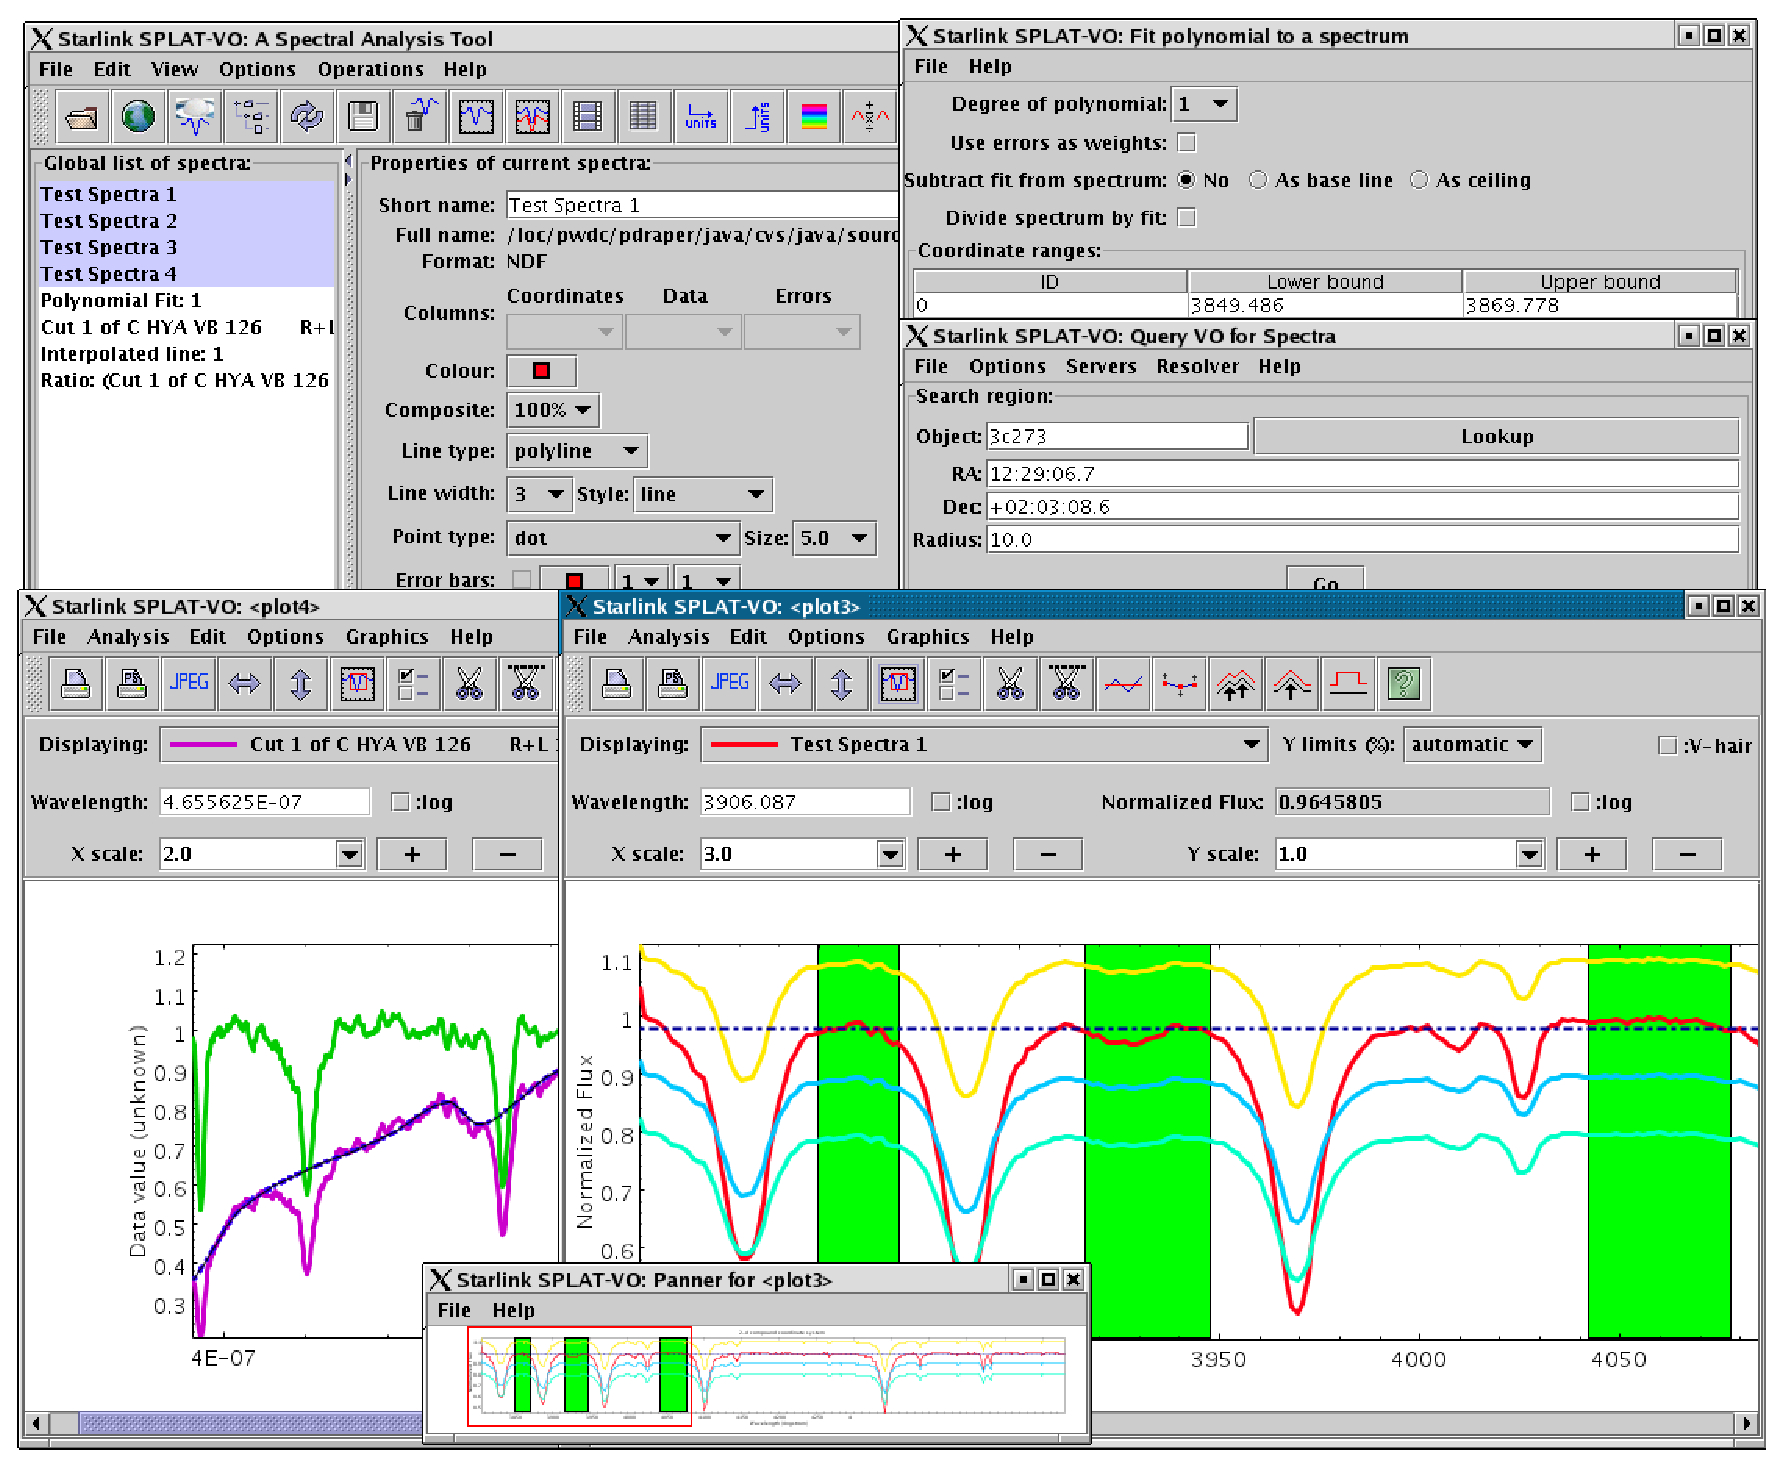
\includegraphics[scale=0.4]{sun243_figures/frontfigure.eps}
\end{center}
% ? End of picture

% ? Heading for abstract if used.
   %\vspace{10mm}
   \begin{center}
      {\Large\textbf{Abstract}}
   \end{center}
% ? End of heading for abstract.
\end{latexonly}

%  HTML documentation header.
%  ==========================
\begin{htmlonly}
   \xlabel{}
   \begin{rawhtml} <H1 ALIGN=CENTER> <FONT COLOR="#000099">\end{rawhtml}
      \stardoctitle
   \begin{rawhtml} </FONT></H1> \end{rawhtml}

% ? Add picture here if required for the hypertext version.
   \begin{center}
      \htmladdimg{frontfigure.jpg}
   \end{center}
% ? End of picture

   \begin{rawhtml} <P> <I> \end{rawhtml}
   \stardoccategory\ \stardocnumber \\
   \stardocauthors \\
   \stardocdate
   \begin{rawhtml} </I> </P> <H3> \end{rawhtml}
      \htmladdnormallink{CCLRC / Rutherford Appleton Laboratory}
                        {http://www.cclrc.ac.uk} \\
      \htmladdnormallink{Particle Physics \& Astronomy Research Council}
                        {http://www.pparc.ac.uk} \\
   \begin{rawhtml} </H3> <H2> \end{rawhtml}
      \htmladdnormallink{Starlink Project}{http://www.starlink.rl.ac.uk/}
   \begin{rawhtml} </H2> \end{rawhtml}
%   \htmladdnormallink{\htmladdimg{source.gif} Retrieve hardcopy}
%      {http://www.starlink.rl.ac.uk/cgi-bin/hcserver?\stardocsource}\\
   \htmladdnormallink{\htmladdimg{source.gif} Retrieve hardcopy}
      {http://star-www.dur.ac.uk/~pdraper/splat/splat-vo/sun243.ps}\\

%  HTML document table of contents.
%  ================================
%  Add table of contents header and a navigation button to return to this
%  point in the document (this should always go before the abstract \section).
  \label{stardoccontents}
  \begin{rawhtml}
    <HR>
    <H2>Contents</H2>
  \end{rawhtml}
  \htmladdtonavigation{\htmlref{\htmladdimg{contents_motif.gif}}
        {stardoccontents}}

% ? New section for abstract if used.
  \section{\xlabel{abstract}Abstract}
% ? End of new section for abstract
\end{htmlonly}

% -----------------------------------------------------------------------------
% ? Document Abstract. (if used)
%  ==================
\begin{center}
\stardocabstract
\end{center}
% ? End of document abstract

% -----------------------------------------------------------------------------
% ? Latex Copyright Statement
%  =========================
\begin{latexonly}
\newpage
\vspace*{\fill}
\stardoccopyright
\end{latexonly}
% ? End of Latex copyright statement

% -----------------------------------------------------------------------------
% ? Latex document Table of Contents (if used).
%  ===========================================
\newpage
\begin{latexonly}
  \setlength{\parskip}{0mm}
  \tableofcontents
  \setlength{\parskip}{\medskipamount}
  \markboth{\stardocname}{\stardocname}
\end{latexonly}
% ? End of Latex document table of contents
% -----------------------------------------------------------------------------

\cleardoublepage
\renewcommand{\thepage}{\arabic{page}}
\setcounter{page}{1}

% ? Main text

\section{Overview\xlabel{overview}}

\SPLAT\ is a graphical tool for displaying, comparing, modifying and
analysing astronomical spectra stored in NDF, FITS and TEXT files as well as
the new NDX format. It can read spectra from local disk files, download them
over the Internet, or it can interact with the Virtual Observatory and query
servers for spectral data in a region of the sky.

\SPLAT\ can handle many spectra at the same time and will display these as
line plots or point markers.
Each display window, of which there can be many, can be used to
view one or more spectra at the same time.
Display windows can be interactively zoomed and scrolled, centred on
specific wavelengths, provide continuous coordinate readout, annotated,
produce printable hardcopy and be configured in many ways.
They also provide the basis for interactive analysis facilities.
All of these functions are displayed in a visually rich format, that
is intended to appeal especially to casual users of spectral data
analysis facilities.

The current set of analysis facilities include background estimation by the
fitting of a polynomial to selected parts of a spectrum or by drawing an
interpolated spline, the fitting of Gaussian, Lorentzian and Voigt profiles to
emission and absorption lines, the filtering of spectra using average,
median and line-shape window functions as well as wavelet denoising and
the calculation of statistics.
A database of laboratory line positions is available to aid in identification.

\SPLAT\ also supports a full range of coordinate systems for spectra,
using the latest facilities of the Starlink \xref{AST}{sun211}{}
library.
This allows coordinates to be \textit{displayed} and \textit{aligned}
in many different coordinate systems (wavelength, frequency, energy,
velocity) and \textit{transformed} between these and different
standards of rest (topocentric, heliocentric, dynamic and kinematic
local standards of rest \etc).
It also uses AST to transform spectra between various flux systems, so that
spectra from a wide variety of sources can be easily compared and used to
produce a spectral energy distribution.
This is an important feature for supporting the heterogeneous data supplied
in the Virtual Observatory.

Finally, \SPLAT\ can interoperate with other VO enabled desktop tools using
the PLASTIC protocol.

% Not advertising this yet. Maybe big changes ahead. Need to make all this
% controlled from the command-line and produce macro replays and scripts.
%  Finally \SPLAT\ is extensible by the use of plugin code and
%  command-line scripts, and can be remotely controlled through
%  SOAP messages and a socket-based mechanism.

If you have any problems with or comments to make about \SPLAT\, then send
these to:
\begin{quote}
\begin{verbatim}
   splat@star.rl.ac.uk
\end{verbatim}
\end{quote}


\section{Getting started\xlabel{getting_started}}

The next two sections describe how to display one spectrum and then
how to display many spectra. If you're new to \SPLAT\ then do take the
time to read these through and try out the example commands.

\newpage
\subsection{Displaying a spectrum}

To start \SPLAT\ you should just need to type the command:
\begin{quote}
\begin{verbatim}
  % splat &
\end{verbatim}
\end{quote}
This assumes that you have \SPLAT\ installed on your system as part of a
standard Starlink installation. If not then you'll need follow any
installation and pre-startup instructions that you have before using
this command.

When \SPLAT\ appears it should look something like:

\mainfigure{browser1}

This is the main \hitext{browser} window. It has a list containing all
the available spectra (in what we call the `global list', but has been
traditionally referred to as the `stack'). Using this window you can
add, save and remove spectra from the list, you can change how a
spectrum draws itself, in all the places that it is shown and make a
spectrum add itself to a plot -- this is how you view spectra.

You can also do things like change the look and feel of the whole
application (there are different colour and font schemes), perform
some quite primitive mathematical operations on or between the
spectra, run through an animated display sequence of some or all of the
spectra, set the spectra coordinate systems and modify/inspect their
values. So things that apply to each spectrum, wherever it is shown,
or the program as a whole are generally done in this window.

To open your first spectrum select the \menuitem{Open} item in the
\menuitem{File} menu. This will create a familiar open file dialogue
window. Just navigate to your spectrum, select it, and press
\menuitem{Open} to proceed.

Alternatively you could have supplied the spectrum you want to use on
the command-line:
\begin{quote}
\begin{verbatim}
  % splat <spectrum_file> &
\end{verbatim}
\end{quote}
Which will read the spectrum stored in the named file. \SPLAT\ will read
spectra stored in most astronomical formats (Starlink NDF, FITS spectra and
tables, simple TEXT files).

Now that you've actually read in a spectrum it will be immediately
displayed in a `plot'. Have a look at this plot window briefly, if you
want, but close it before proceeding (to close it select the
\menuitem{Close} item in its \menuitem{File} menu). You really need to
understand how to display a spectrum in a plot yourself, if you're to
gain complete control over the creation of plots and what they
display.

The browser window (once again on its own) should now appear something
like:

\mainfigure{browser2}

Now to re-create a plot and display a spectrum in it the hard
way. Actually this couldn't be simpler, just `double click' on the
name in the \labelitem{Global list of spectra}. Another way to achieve
the same effect is to \hitext{select} the name (by just clicking on it
once, you can tell it's selected when it becomes highlighted, as shown
above) and choose the display selected spectra button in the
toolbar. This is the button that looks like \inline{display} (it's
meant to represent a spectrum with axes drawn in a plot). If you're
successful then a window looking like this:

\mainfigure{plot1}

should appear as before.

Since \SPLAT\ is meant to be capable of displaying many spectra
(sometimes in the same plot as we'll see in the next section), you
should confirm this by creating a second plot window, by just
performing the same operation again (\ie\ double click on the
spectrum name).

\newpage
\subsection{Displaying more than one spectrum\xlabel{displaying_more_than_one_spectrum}}

Displaying many spectra at the same time isn't much more difficult
than the single spectrum case. Just open up several spectra by giving
their names on the command-line, or by opening them using the
\submenuitem{File}{Open} dialogue. This will produce a main window that
looks something like:

\mainfigure{browser3}

If you've opened all the spectra at once (you can do this using the
\submenuitem{File}{Open} dialogue by selecting more than one file --
just hold down the shift key while selecting each one) then they will
have also all appeared displayed in a single plot, which should look
something like:

\mainfigure{plot2}

Again you should now close the plot (or all the plots if you've opened
the spectra one-by-one) so you can find out how to add spectra to
plots manually.

There are three ways to display a set of spectra in a single plot, you
can either open a plot just displaying one spectrum and then add the
others one-by-one, by two different methods, or you can open a plot
displaying a pre-selected list of spectra. Let's cover the latter
option first.

\label{selecting_spectra}
The first thing to do is identify which spectra you want to display in
the same plot, you do this by selecting their names in the
\labelitem{Global list of spectra:} list. You can select more than one
name at a time by holding down the control key, while clicking on the
name. It's also possible to select ranges of names by selecting the
first name and then selecting the last name while holding down the
shift key. Have a play to see the effects that you can get with
combinations of these (hint: using the control key also allows you to
remove single names from the selection). To select all the names you
can also use the \submenuitem{Edit}{Select all spectra} menu item.

Now that you've selected the spectra to display, just press the
multi-display button: \inline{multidisplay} and all the spectra
will be displayed in a single plot. Note that if you inadvertently
press the single display button: \inline{display}, then each
spectrum will appear in a plot of it's own (this can be a very bad
idea if you have a very large number of spectra selected!).

If you don't like the colours chosen for your spectra you can just press the
auto-colour button: \inline{rainbow} to get a new set. Each press of this
button should generate a new set of colours, so just keep clicking until you
see a combination that you like.

The second method for adding more than one spectrum to a plot is the
simplest, you can drag spectra from the \labelitem{Global list of
spectra:} and drop them into the display area of the plot. To drag a
single spectrum just make sure that it is selected and then attempt to
drag it from the \labelitem{Global list of spectra:} into the plot
(during dragging a document icon should be attached to your screen
pointer). To drag more than one you just need to make all the spectra
you want displayed selected and then attempt to drag any of the
selected set.

The third method is actually also the method you'd use to remove a
spectrum from a plot. The first thing to do is select a spectrum in the
\labelitem{Global list of spectra:},
this shows its properties in the
\labelitem{Properties of current spectra:}
side of the browser window, including which views
are being made (\ie\ which plots are displaying it). To add or remove
a spectrum from a plot you need to click on the square shown in the
\labelitem{Displayed} column, so that it becomes ticked or unticked. See
in the following image that \hitext{test spectrum 2} is currently
being displayed in \hitext{<plot0>}:

\mainfigure{browser4}

If any spectra were not displayed in this plot then they could be
added to it using this mechanism. Naturally this also extends to the
case when there are many plots available.

\newpage
\subsection{Basic control of a plot view\xlabel{basic_control}}

The final part of this introduction is to zoom and scroll the
spectrum, so, for instance, you can inspect individual lines and read
off accurate coordinates (this is after all the main purpose of
\SPLAT).

Zooming of a plot is controlled by the \labelitem{X scale:} and
\labelitem{Y scale:} controls. To adjust the zoom you may either select a
value from the drop-down lists, or you may type in a value and press
\hitext{<Return>}. Values may be non-integer, but should be one or more.

Once you have zoomed the plot scrollbars should appear at the bottom
and maybe to the right (these appear when the size of the plot becomes
larger than its visible size). Just drag the slider from side-to-side
or up-and-down to view the part of the plot that you want to see.

\mainfigure{plot4}

A useful shortcut for zooming is to drag out a region using the middle
mouse button. Just place your cursor on the plot, press the middle
button and, keeping the button depressed, move the mouse until the
rubber-band rectangle encloses the feature you want to zoom on. You
can also zoom in by an increment of one in X and Y by pressing the
middle button and just releasing it.

If you find that the figure is zoomed so much that you're having
difficulty recognising the features, then there are several things
that you can do.

The first is to resize the plot so that it has a scale of 1 in X or
Y. That's what the toolbar buttons that appear as
\inline{fitwidth} and \inline{fitheight} do, make the plot scale its
displayed spectra to fit the visible width or height.
\textbf{Note:} These buttons are very useful when a plot seems to be
displaying nothing or reports that the plot has no size etc., they are your
best friends, press them a lot in such circumstances.

If what you really want to do is remain zoomed but quickly go to a
given wavelength, then all you need to do is type in the wavelength in
the X-coordinate readout entry field (labelled \labelitem{Wavelength}
above), press \hitext{<Return>} and the plot will be centred (or
brought into the edge of the field of view).

If what you'd really like is a smaller view of the whole plot to work
from, then press the \inline{panner} button, this will pop-up the
`panner'. This shows a red rectangle over a view of the full unzoomed
plot (shown in the same aspect ratio as the full plot at the current
scale factors). To move the rectangle, and hence the view shown in the
plot, just point somewhere in the panner and press the left mouse
button, or `drag' the rectangle itself.

If the panner view seems very small, as can happen when you're using a
high X scale factor, then try resizing the window to get a better fit
to the aspect ratio (hint: make it taller).

\mainfigure{pannerwindow}

\section{Help for individual windows\xlabel{help_window_individual}}

The following sections are descriptions of how to use the
\SPLAT\ windows, hopefully these should only serve as reference
material, the function of windows should be clear from their
descriptions, balloon-help and context. Use a window's \menuitem{Help}
menu to view its related page on-line.

\newpage
\subsection{The browser window\xlabel{browser_window}}

The browser window has several main elements, each of which is shown
in the following figure:

\mainfigure{browser5}

\subheading{Global list of spectra}
\begin{quote}
 In the \labelitem{Global list of spectra} short names for each
 spectra are shown. The short names are intended to allow the quick
 identification of spectra and can be modified at any time by
 selecting the name and then typing a new name in the
 \labelitem{Short name} field (remember to press \hitext{<Return>} to
 make the change happen). Initially short names are read from the
 \hitext{TITLE} or \hitext{OBJECT} properties of spectral data formats
 that support these (\ie\ NDF and FITS respectively), otherwise they
 default to the file name.

 Another important concept related to the global list, is using it to
 create a selected range or list of the spectra. Selection is
 important as this identifies which spectra you'd like to see
 properties for, or want to work with. There's a quick tutorial on
 \htmlref{selecting spectra}{selecting_spectra} in the introductory material
 \latex{(\S\ref{selecting_spectra})}.
\end{quote}

\subheading{Properties of current spectra}
\begin{quote}
 In the properties area there are controls for changing how the currently
 selected spectra are displayed (a spectrum always uses the same display
 properties) and where they are displayed.

 If more than one spectrum is selected then the properties shown are those of
 the first spectrum (\ie\ highest in the global list). However, any changes
 that you then make are applied to all the selected spectra.

 If you load a table into \SPLAT\ the \labelitem{Columns:} controls will show
 the names of the columns selected. If these are incorrect then you can choose
 a different set.

 The properties that you can change include the colour (press on this to get a
 swatch of selectable colours), the composite value (that is the transparency
 so you can see lines or points through other line or points), the line type
 (simple connected polyline or histogram, or just a point marker). If you
 choose to draw lines then you can set the width and style (dashed \etc). If
 you choose to draw points then various types are available.

 If the selected spectra have errors then you can display error bars by
 clicking on the \labelitem{Error bars:} control. This is greyed out if errors
 are not available. The colour, number of sigma drawn and frequency of the
 error bars can be changed using the other controls on this line.

\end{quote}

\subheading{Views of current spectra}
\begin{quote}
 The views of the current spectra region shows the names of the plots that are
 displaying the currently selected spectra (this time if a plot is showing
 only some of the spectra, then it is highlighted in red). To add a spectrum
 or list of spectra to a plot, select their names in the global list and then
 click on the \labelitem{Displayed} control (normally this results in a tick
 appearing). If a plot is already displaying some of the selected spectra then
 you force it to display them all by clicking twice -- the first click removes
 the selected spectra and the second puts them all back, plus the ones not
 already shown.

 To make a plot visible double click on its name. This should raise and
 deiconify it.
\end{quote}

\subheading{Toolbar and menus}
\begin{quote}
 The toolbar region has a series of buttons that act as short-cuts to
 many of the functions found in the main menus. Here's a quick break
 down of what they do:
 \begin{itemize}

  \item[\inline{openfile}] Create an open file dialogue. You can use this
  to browse any local files and select a list of them for opening. When
  opened they are added to the global list and displayed in a new plot
  (unless you untick the \labelitem{Display} control). You may open files
  that are already in the global list, this just creates a new entry.
  Normally the type of a spectrum is determined using the file extension,
  but using this dialogue you can select a type, or ask that it be guessed.

  \item[\inline{location}] Download and display a spectrum from the Internet.
  If you have a URL for a spectrum to view then use this simple dialog.

  \item[\inline{ssap}] Query any known Simple Spectral Access Protocol (SSAP)
  servers about spectra that they hold on a region of the sky and download
  these to \SPLAT. This tool provides access to the Virtual Observatory.

  \item[\inline{browse}] Browse a hierarchy of files. This dialogue can be used
  like the open file dialogue to choose a file containing a spectrum, but,
  it also allows you to look inside a file for any displayable components.
  This is useful for FITS files that contain extensions (spectral or table
  extensions can be opened), or HDS files that contain more than one NDF.
  The file type guessing used here is the same as that used when you set
  a type of \hitext{guess} (either on the command-line or by using the
  open file dialogue).

  \clippedmainfigure{treeview}

  \item[\inline{reopen}] Re-open the selected spectra. If the files containing
  your spectra change on disk you can select them in the global list get them
  opened. Note that not all spectra are backed by a suitable disk-file, these
  types will be ignored.

  \item[\inline{savefile}] Create a save file dialogue. Using this you can
  save a spectrum to disk-file. There are no restrictions on which file
  format you can save to, but information may be lost for certain types
  (\ie\ TEXT format).

  \item[\inline{remove}] Remove the currently selected spectra from the
  global list. This does not modify disk files. Spectra that are only
  resident in memory will be lost, without warning.

  \item[\inline{display}] Display the currently selected spectra in
  plots. Each of the selected spectra is displayed in a plot of its
  own. A similar effect is obtained by double-clicking a spectrum in the
  global list.

  \item[\inline{multidisplay}] Display all the currently selected
  spectra in a single plot. Use this when you want to compare spectra.

  \item[\inline{animate}] Open a window to control the animation of some
  of the spectra. Using this window you can also create a JPEG or PNG
  sequence of the animation.

  \item[\inline{table}] View and possibly modify the coordinates and
  data values of the selected spectra. This shows an editable table of
  values. It is also possible to make global changes using
  algebraic expressions to convert or create new values.

  \item[\inline{xunits}] Open a window to set or remap the coordinate
  systems of any of the spectra. A variety of systems can be used
  covering wavelength, frequency, energy and velocity. Unit
  information can be used to align spectra in a plot (so you can
  trivially compare spectra in say angstroms and nanometres,
  energy and frequency or even heliocentric and topocentric rest frames
  \etc).

  \item[\inline{yunits}] Open a window to set the data units of any spectra.
  This can be useful when just setting the units displayed in a plot, but
  can also be used to convert spectra between flux systems when they are
  drawn (making them correctly aligned).

  \item[\inline{fits}] View the FITS headers of any selected spectra.
  A window displaying the headers will be opened for each of the selected
  spectra. Note that only 1D FITS and NDFs will generally have FITS headers
  other types, including FITS tables, will not.

  \item[\inline{rainbow}] Change the colour of \hitext{all} the spectra
  in the global list. Each time you press this button a new random seed
  is used to generate a different sequence of colours, so keep pressing
  until you see a sequence you like.

  \item[\inline{binarymath}] Perform simple maths (add, subtract, divide
  and multiply) between pairs of spectra.

  \item[\inline{unarymaths}] Perform simple maths using a spectrum and a
  constant (add, subtract, divide and multiply).

  \item[\inline{help}] Access the on-line help system.

\end{itemize}

 Interesting menu items not found in the toolbar are a list of standard line
 position catalogues (for optical and some IR and submillimeter lines), these
 are found in \submenuitem{Options}{Line identifiers}.  Others are to do with
 controlling the selection of the spectra and plots (see the \menuitem{Edit}
 menu, just like deleting spectra from the global list you can delete all the
 selected plots) and changing the `look and feel' of \SPLAT. These options are
 found in the \submenuitem{Options}{Look and Feel} and
 \submenuitem{Options}{Colour Theme} sub-menus. Note that if you select the
 CDE/Motif look and feel you cannot change the colour and fonts used.

 You can also save and restore the global stack of spectra to and from
 diskfile using a special data format that is only recognised by \SPLAT.
 Using this method allows you to save a working set of spectra and restart an
 analysis later. Properties such as the line colours are restored, but any
 relationship between disk files and the spectra in the global list is
 lost. Data saved in a stack are compressed.

 The \menuitem{Interop} menu contains items for communicating with other 
 PLASTIC-aware desktop applications. This is described in the 
 \htmlref{Tool interoperability using PLASTIC}{plastic} section
 \latex{(\S\ref{plastic})}.

 Finer control of the initial coordinate system picked by \SPLAT\ is given by
 the \submenuitem{Options}{Find spectral coordinates} menu item.  When this is
 selected (the default), \SPLAT\ will check for any spectral coordinate system
 in the input spectra and use that, if the default coordinate system isn't
 spectral. It will also use any units it can locate to attempt a guess if all
 else fails. Unfortunately this means that if you intend to view another
 coordinate system (like GRID to see the channel numbers), it might fail, so
 switching this off gives you complete control. This option can also be
 enabled using the \verb+-k,--keepcoords+ switches on the command-line.

\end{quote}

\subheading{Accelerator keys}

\begin{itemize}
\item \labelitem{Control-o} Activate open file dialog.
\item \labelitem{Control-l} Activate location dialog.
\item \labelitem{Control-r} Re-open all spectra.
\item \labelitem{Control-w} Close window (and exit application).
\item \labelitem{Delete} Remove selected spectra.
\item \labelitem{Control-a} Select all spectra.
\item \labelitem{Control-d} Display selected spectra in plots.
\item \labelitem{Control-i} Display selected spectra in same plot.
\item \labelitem{Control-u} Re-colour all spectra.
\item \labelitem{Control-p} Register with PLASTIC server.
\item \labelitem{F1} Display help on \SPLAT.     
\item \labelitem{Shift-F1} Display help on window.
\end{itemize}

\newpage
\subsection{A plot window\xlabel{plot_window}}

The anatomy of a plot window is shown below:

\mainfigure{plot3}

It has three main regions, the menubar \& toolbar, the control panel and
the display area.\\

\subheading{The display area}
\begin{quote}
 The display area shows a view of all the spectra that are currently
 associated with this plot. The colours, plotting style \etc\ of these
 spectra are determined by their global properties as set in the main
 browser window.

 The plot title and axis labels are determined using the properties of the
 current spectrum, if possible. For instance if the current spectrum is an NDF
 then these values are determined from the NDF's title, units and axis
 components, or for more recent NDFs from the properties of its WCS
 component. Similarly for FITS files these values are determined using the
 world coordinates FITS keywords. To change these look in the
 \labelitem{Configure Plot Options} window, which is activated by pressing the
 \inline{config} button.

 The size of the area used to display a spectrum is initially determined from
 an automatic match of its data and coordinate extents to the visible surface
 of the display area, you can change the size of the display surface using the
 zoom controls described below and/or you can change the actual data limits
 using the \labelitem{Configure Plot Options} window. When you add or remove a
 spectrum the apparent size of the display region stays the same and all the
 spectra now displayed are scaled to fit within it. To return to a state where
 the visible surface matches the display area you need to press the
 \inline{fitwidth} and \inline{fitheight} buttons.

 The \labelitem{Configure Plot Options} window also offers the ability change
 the colour of the display area background, to draw the lines using
 anti-aliasing (which reduces the jagged effects, but at the cost of drawing
 speed), to modify the reserved area around the plot and do things like
 position the numeric labels, set the axis gaps \etc\

 The following interactions are provided in the display area.
 \begin{itemize}

  \item Continuous coordinate and data readout: when you move the mouse
  pointer over the display area the coordinates and data value of the nearest
  point of the current spectrum are shown in the control panel.  If the
  readout is not updating you have probably moved outside of the extent of the
  current spectrum (the one selected in the \labelitem{Displaying:} control).

  If the vertical hair is enabled, then this also follows the mouse
  pointer.

  \item Region Zoom: you can zoom on a feature by dragging a rectangle
  over it using the middle mouse button.

  \item Incremental Zoom: you can increase the zoom factors by one
  simply by pressing the middle mouse button anywhere in the display
  area or pressing the $\_/=$ keys. If you hold down the shift key
  these zoom in Y, otherwise in X.

  \item Scrollbars: when the X or Y zooms make the plot greater in size
  than the display area scrollbars appear to the bottom and right. Just
  drag the sliders to scroll.

  \item Keyboard Scroll: the arrows keys can be made to control the
  scroll, provided the keyboard focus is in the display area. Make sure
  of this by clicking the left mouse button while pointed in the display
  area.

  \item Interpolated data value: if the keyboard focus is in the
  display area and the vertical hair is shown, then pressing the space
  bar will display the interpolated position of the hair, rather than
  the X coordinate and data value of the nearest position in the
  spectrum.

  \item Interactive graphics control: if any interactive graphics figures are
  shown (such as those that define ranges for fitting backgrounds and spectral
  lines, or are produced by the controls in the \menuitem{Graphics} menu),
  then these can be moved by selecting them (just click on one and little
  grips appear around the edges) and then dragging them and resized by
  dragging the edge grips.

  \item Drop target: you can drop any spectra dragged from the global
  list and they will be displayed.

 \end{itemize}
\end{quote}

\subheading{The control panel}
\begin{quote}
 The control panel area provides controls for interacting with the
 plot. It also shows details of what spectra are displayed in the plot
 and a continuous readout of the X coordinate and corresponding data
 value.

 The \labelitem{Displaying:} drop down list shows the names and current
 rendering properties of any spectra that are displayed. If you choose a
 spectrum from this list it becomes the \labelitem{current spectrum} and is
 used as the basis for the plot's coordinates (so the readouts now show the
 values of this spectrum, also the plot will be re-drawn if the coordinate
 system of the newly selected spectrum is different). The selected spectrum
 also becomes selected in the browser window (so you see its details more
 clearly and apply modifications). This spectrum is also the one used by any
 tools (such as background and line fitting) that work with only one
 spectrum. If you remove this spectrum using the \submenuitem{Edit}{Remove
 current spectrum} option then the next spectrum in the list becomes the
 current one.

 The \labelitem{Y limits (\%):} drop down list provides a series of
 quick cuts for setting the limits of the Y axis. Normally this is the
 full range, but using a percentage cut can usefully clip the range to
 reject extreme outlier data values. The data values used are restricted
 to the limits of then X coordinates (all when automatic ranging is used, 
 the default ).

 The \labelitem{Wavelength:} entry control has two functions. The
 first is to show the current wavelength. The second is to allow you
 to centre the display area on a specific coordinate. Just type in the
 value you want to see here and press \hitext{<Return>}. Note that the
 label of this area modifies to match the label of the X axis, so
 could say something different to \labelitem{Wavelength:}.

 The \labelitem{:V-hair} checkbox controls whether the `vertical hair'
 is shown. The vertical hair is just a vertical line that follows the
 mouse pointer around the display area. It can be quite slow, so isn't
 shown by default.

 The \labelitem{X scale:} and \labelitem{Y scale:} controls change the
 zoom of the display area. The plus and minus controls increase and
 decrease the zoom by one, or you can choose a zoom from the drop-down
 lists, or you can type in a decimal value (which should be greater
 than equal to one) and press \hitext{<Return>}.

 The \labelitem{:log} controls determine if either of the axes are drawing
 using log spacing (this is not possible if either axis spans the value
 zero). Finer control of the log spacing and labelling can obtained using the
 plot configuration window.

 The \labelitem{Track free} checkbox determines what values are shown in the
 continuous coordinate readouts. When unchecked (the default) the values
 shown are the nearest ones of the current spectrum to the pointer position.
 When checked the readouts show the coordinates under the pointer.

\end{quote}

\subheading{Toolbar and menus}
\begin{quote}
 The toolbar region has a series of buttons that act as short-cuts to
 most of the functions found in the main menus. Some of these create
 new windows with complex actions that should be consulted for further
 help.

 \begin{itemize}

  \item[\inline{print}] Print a copy of the display area to an installed
  printer or to a file. The output produced fits the output page format using
  the current aspect ratio of the display area, so if you're zoomed by a large
  factor then you'll get an output page that has a very small height. If you
  want a printout of just the visible part then cut it out and display it in a
  new plot first. Postscript output from this dialogue isn't encapsulated.
  The next figure is an example of this output. Note that if you're looking at
  a paper copy of this document you're looking at the postscript output and if
  you're looking at the on-line help it shows a scaled JPEG for on-line copies
  (see item after next).

  \clippedmainfigure{printoutput}

  \item[\inline{postscriptprint}] Same as the print option, except, this only
  offers to write a postscript file and doesn't rely on having any printers
  installed on the local machine. The output can be in encapsulated form
  for inclusion in other documents.

  \item[\inline{jpegpng}] Make a JPEG or PNG image version of the display
  area. Again the file produced fits the output graphic using the current
  aspect ratio of the display area. The default is to produce an image
  with a pixel-to-pixel correspondence to what you see on the screen
  (if it were possible to view the whole of the area). Alternatively you
  can scale the graphic to fit some dimensions that you enter, or just
  clip the graphic to these dimensions. (Hint: if you want anti-aliased
  lines drawn in the image select this plotting option first using the plot
  configuration window).

  \item[\inline{fitwidth}] Make spectra fit the display area width.  Use this
  to quickly return to an unzoomed coordinate state and to match the X axis
  width when you resize the plot window.

  \item[\inline{fitheight}] Make spectra fit the display area height.  Use
  this to quickly return to an unzoomed data value state and to match the Y
  axis height when you resize the plot window.

  \item[\inline{panner}] Show the `panner' window. You can use this to
  see a view of the whole extent of the currently displayed spectra
  (shown at the same aspect ratio as the display area). This also
  features a red rectangle that shows the extent of the display area,
  this can be moved to change the display area view.

  \item[\inline{config}] Show the plot configuration window. This
  contains many controls for setting the display area data limits,
  changing the plot title and axis labels, drawing grid lines,
  defining how many ticks to display, changing the amount of space
  around the plot edges, setting the background colour and whether to
  draw text or text and lines using anti-aliasing. It also offers
  facilities to save these settings for future restoration.

  \item[\inline{cutter}] Create a new spectrum (on the global list)
  that contains only the visible parts of the current spectrum. You
  can then display this new spectrum in this or a new plot. The new
  spectrum is given the name \hitext{Cut <n> of <current\_shortname>}.
  This facility is useful to create printouts of just parts of a
  spectrum and to speed up processing of very large spectra.

  \item[\inline{regioncutter}] Show the region cutter window. This
  window allows you to graphically define which regions you'd like to
  cut or delete from the current spectrum.

  \item[\inline{fitback}] Show the toolbox for fitting a polynomial to
  defined regions of the current spectrum. This is used to define
  backgrounds prior to line fitting, or for subtracting and dividing
  backgrounds from spectra.

  \item[\inline{interpolate}] Show the toolbox for taking an interpolated
  curve (\ie\ a spline drawn on the plot using the features of the
  \labelitem{Graphics} menu) and creating a spectrum from it.

  \item[\inline{fitline}] Show the toolbox for fitting emission and absorption
  lines. This measures the line position and equivalent width as well as
  fitting Gaussian, Lorentzian and Voigt profiles to selected wavelength
  ranges of the current spectrum. Remember to define a polynomial background
  before using this tool or have your data processed for fitting.

  \item[\inline{filter}] Show the toolbox for filtering the current
  spectrum. The filters offered are simple ones like the average and
  median over a windowed area, plus more complex ones like smoothing
  using any of the known line shapes and denoising using wavelet
  transformations.

  \item[\inline{units}] Show the toolbox for selecting new coordinates or
  data units for the current spectrum (and therefore plot).

  \item[\inline{flip}] Show the toolbox for flipping, shifting or redshifting
  editable spectra shown in the plot. Also allows you create an editable copy
  of the current spectrum.

  \item[\inline{sigma}] Show the toolbox for determining statistics (mean,
  standard deviation, \etc) of the whole or parts of the current spectrum.

 \end{itemize}

 The \menuitem{Options} menu contains several control items whose values are
 preserved between invocations of \SPLAT.

 \begin{itemize}

  \item \submenuitem{Options}{Match coordinates and/or fluxes}.
  When this is selected the plot will attempt to convert the spectral
  coordinates and fluxes of all displayed spectra into the systems of the
  current spectrum, so that they will be aligned when displayed.

  Whether this works or not depends on whether the spectra that you have read
  in contain correct descriptions (or descriptions that \SPLAT\ can make good
  guesses about) of the spectral coordinates and data fluxes and whether the
  flux system is supported. If this doesn't work then check that your spectra
  have valid descriptions using the toolboxes in the main browser window for
  inspecting and setting spectral coordinates and data units
  (\inline{xunits} and \inline{yunits}).

  In the case of line identifier catalogues, these will also be transformed to
  the rest frame of the observed source (\ie\ they will be red or blue shifted
  if you have defined the source velocity as part of its coordinate system
  definition).

  This option is switched on by default. If your spectra do not need aligning
  switch if off for extra performance.

  \item \submenuitem{Options}{Match non-flux data units}.
  If your data units are not understood as fluxes it may still be possible to
  align them (dimensionally obvious unit conversions are possible for instance
  mK and K will be aligned correctly, as will eV and keV).

  \item \submenuitem{Options}{Match sidebands}
  If your spectra are dual sideband then they can be aligned taking this 
  into account, or they can be aligned just using the currently selected
  sidebands. By default they are not aligned by taking the sideband into 
  account.  If you want to do otherwise select this item.

  \item \submenuitem{Options}{Match origins}
  If you have defined origins for your spectra to display offset coordinate
  systems then selecting this will align the spectra in those coordinates
  not the absolute ones.

  \item \submenuitem{Options}{Match using base system}
  When matching spectra it is usual to achieve this by transforming all
  coordinate systems into a common system, this system is wavelength by
  default. For some systems it may be better to use another common system
  so by selecting this option you can set the common system used to be that of
  the current spectrum. This option is most useful when working with
  velocities, when you want the alignment to happen in that system 
  (because the spectra have different rest frequencies).

  \item \submenuitem{Options}{Only display grid axes in visible area}
  Normally the labelled axes displaying the spectral and data coordinates are
  drawn to the full size of the display surface of the plot. This is the
  quickest mode as it reduces the need for re-drawing. If you select this
  option the axes will be only drawn within the the visible part of the plot,
  which makes it easier to see the coordinate labels, but means that the axes
  need to be re-drawn continually when scrolling.

  \item \submenuitem{Options}{Only display spectra within axes}
  Select this option if you only want spectra (including line identifiers) to
  be drawn within the bounds of the axes. When combined with the previous
  option to only display axes in the visible area this will potentially slow
  down scroll operations a lot, so the default is off.

  \item \subsubmenuitem{Options}{Line identifiers}{Load all matching line identifiers}
  If you select this option then all line identifiers known to \SPLAT\
  (including any that you have opened yourself), and whose coordinate ranges
  fall within that of the plot, will be loaded into the global list and
  displayed in the plot. Note that this will not work if the spectra displayed
  in the plot do not have defined spectral coordinates.

  \item \subsubmenuitem{Options}{Line identifiers}{Load all matching pre-loaded line identifiers}
  If you select this option then all line identifiers already loaded into the
  global list, and whose coordinate ranges fall within that of the plot, will
  be displayed in the plot. Note that this will not work if the spectra
  displayed in the plot do not have defined spectral coordinates.

  \item \subsubmenuitem{Options}{Line identifiers}{Positions track current spectrum}
  If you select this option then line identifiers that do not have data
  positions (this is typically true) will be positioned above the current
  spectrum, rather than displayed in a line along the bottom of the plot.

  \item \subsubmenuitem{Options}{Line identifiers}{Prefix name to labels}
  If you select this item then the short name of each line identifier spectrum
  displayed in the plot will be prefixed to the label. This allows you to
  discriminate between crowded labels. Note that the short name of a line
  identifier can be modified in the main window, once it is loaded into the
  global list. For legibility any names that are appended by
  \labelitem{\_lines}, will have that string removed and any underscores will
  be replaced by spaces.


  \item \subsubmenuitem{Options}{Line identifiers}{Draw horizontal labels}
  Select this option if you want line identifier labels drawn horizontally
  rather than vertically.

  \item \submenuitem{Options}{Error bar auto-ranging}. When auto-ranging a
  spectrum that has associated errors the limits do not include the extent of
  any error bars that will be drawn, if you want this to be otherwise select
  this option.

  \item \submenuitem{Options}{Draw errors as spectrum}. If this option is
  selected and any of the displayed spectra have errors, then those spectra
  with errors will be drawn using the error value as each point on the line
  rather than the data values (and conversely the data values will be used to
  draw error bars, if that is enabled for any of the spectra). When displaying
  spectra without any errors this option has no effect.

  \item \submenuitem{Options}{Auto-fit percentiles in Y}. When this option is
  selected choosing a percentile limit in Y results in the plot also being
  forced to fit the height of the plot.

  \item \submenuitem{Options}{Short names in menu lists}. When this option is
  deselected the long names (usually file names) are shown in the
  \label{Displaying:} drop-down menu.

 \end{itemize}
\end{quote}

\subheading{The Graphics menu}

The \menuitem{Graphics} menu provides methods for drawing text and a range of
figures on the plot. This allows you to add annotations, but also provides the
basis for the interactive graphics used by the various toolboxes.

To draw a figure on a plot you need to select an option from the
\menuitem{Drawing mode} sub-menu and then, depending on the figure type, either
drag out a region or select fiducial points. When creating a figure using
points these are completed using a double click on the last point.

In the \menuitem{Drawing mode} menu the currently available figure types are:
\begin{quote}
\begin{itemize}
  \item[\inline{line}] a straight line,
  \item[\inline{rectangle}] a rectangle,
  \item[\inline{ellipse}] an ellipse,
  \item[\inline{polyline}] a poly line (last point not connected to first),
  \item[\inline{polygon}] a polygon (last point connected to first),
  \item[\inline{freehand}] freehand curve,
  \item[\inline{text}] a text string,
  \item[\inline{curve}] an interpolated curve (splines and special spectral
                        shapes),
  \item[\inline{xrange}] a rectangle which only moves along X (indicates a
                         range of coordinates).
\end{itemize}
\end{quote}

There are also two special modes:
\begin{quote}
\begin{itemize}
  \item[\inline{select}] select figure,
  \item[\inline{edit}] edit figure.
\end{itemize}
\end{quote}
When the mode is select (this is usually the default state), clicking on a
figure selects it. You can then drag it around to move it, or drag one of the
grips (the little squares) to change the shape. To select more than one figure
you hold down the \hitext{<Shift>} while clicking.

The edit mode can be used to add new points to a polyline, polygon or
interpolated curve. Just select this, click on the figure you want to edit and
then start adding new points. You can also edit text strings, just choose the
edit mode and click on the text, this produces a dialogue with the text for
editing.

To change the properties of a figure (line width, fill/outline colour, font
\etc) just select the figure and then choose the option you want to change
from the various menus. You can define these before creating a figure too.

Interpolated curves are like polylines in that they are defined by a series of
points, but they can only have increasing or decreasing X coordinates (so
cannot double back on themselves). They are intended for drawing figures that
are related to spectra, specifically spectral backgrounds and lines. In fact
if you draw an interpolated curve you can convert it into a spectrum for
removing from a real spectrum using the \labelitem{Generate spectra from
interpolated lines} toolbox. The types of interpolation scheme available are:
\begin{quote}
\begin{itemize}

  \item Hermite, interpolation based on Hermite polynomials. The effect is
        supposed to construct reasonable analytic curves through discrete data
        points (\ie\ like those a human would produce).

  \item Akima, interpolation based on Akima splines. Like Hermite this
        supposed to construct human-like analytic curves.

  \item Cubic, interpolation using natural cubic splines.

  \item Polynomial, interpolation using a simple polynomial of order one less
        than the current number of points.

  \item Linear, interpolation using straight-lines (like polyline, except it
        has sorted X coordinates).

  \item Gaussian, interpolation using a Gaussian line-profile. This can only
        have four reference positions (and is initialised from the first two
        indicated on the plot), these define the left extent, width,
        height/centre and right extent. The order will switch if these are
        dragged past each other (so dragging the width grip beyond the left
        extent grip will switch their meaning).

  \item Lorentz, interpolation using a Lorentzian line-profile. Works like the
        Gaussian curve.

  \item Voigt, interpolation using a Voigt line-profile. This also works like
        the Gaussian curve, but has five characteristic positions, left
        extent, Gaussian width, height/centre, Lorentzian width, right extent.

\end{itemize}
\end{quote}

Once you have created your figures you may want to save them for restoration
at a later time, this can be done using the
\submenuitem{Graphics}{Save/restore figures} dialogue. Figures are saved using
the physical coordinates of the spectrum, so should be re-drawn at the correct
wavelengths \etc\ on new plots.

\subheading{Accelerator keys}

\begin{itemize}
\item \labelitem{Control-p} Activate print to printer dialog.
\item \labelitem{Control-t} Activate print to postscript file dialog.
\item \labelitem{Control-j} Activate print to JPEG file dialog.
\item \labelitem{Control-b} Scale spectrum to fit visible width.
\item \labelitem{Control-h} Scale spectrum to fit visible height.
\item \labelitem{Control-a} Show the panner window.
\item \labelitem{Control-o} Show the plot configuration window.
\item \labelitem{Control-w} Close the window.
\item \labelitem{Control-v} Cut out the current view of the spectrum.
\item \labelitem{Control-r} Activate cut out regions of spectrum window.
\item \labelitem{Control-y} Activate fit polynomial to background window.
\item \labelitem{Control-g} Activate generate spectrum from drawn curve window.
\item \labelitem{Control-l} Activate fit spectral lines window.
\item \labelitem{Control-f} Activate filter spectrum window.
\item \labelitem{Control-u} Activate quick change units window.
\item \labelitem{Control-l} Activate flip compare window.
\item \labelitem{Control-s} Activate statistics window.
\item \labelitem{Control-[1-9]} Select drawing mode for various graphics figures.
\item \labelitem{Delete} Delete any selected graphics figures.
\item \labelitem{Shift-Delete} Delete all graphics figures.
\item \labelitem{r} Raise any selected graphics figures.
\item \labelitem{l} Lower any selected graphics figures.
\item \labelitem{h} Hide or unhide all graphics figures (toggle).
\item \labelitem{F1} Display help on \SPLAT.     
\item \labelitem{Shift-F1} Display help on window.
\end{itemize}



\newpage
\subsection{The query VO for spectra window{\xlabel{ssap_window}}}

This window provides basic access to the Virtual Observatory. Using it you can
query the current list of SSAP servers (Simple Spectral Access Protocol) for
lists of the spectra that they hold about a circular region on the sky. You
can then select which of these you are interested in and download these into
\SPLAT.

\mainfigure{ssapwindow}

The figure above shows the window after a query to all the currently known
servers has been made.

To lookup the coordinates of an object just type in an identifier in the
\labelitem{Object} field and either press \hitext{<Return>} or the
\labelitem{Lookup} button. Alternatively if you know the coordinates
(FK5/J2000) of the region of sky you can just enter the coordinates in the
\labelitem{RA} and \labelitem{Dec} fields. 

The \labelitem{Radius} value is a number of arcminutes to search about the
position. The \labelitem{Band} entries define a lower and upper limit, in
meters, for the spectral bandpass (not all SSAP servers support this option,
those that do may offer just an upper limit and allow you to set a wavelength
to include by setting just a lower limit).

Once you have identified the region to search press the \labelitem{Go} button
to contact the current list of SSAP servers. To make these queries it may be
necessary for you to tell \SPLAT\ about your local web-proxy server (this is
the same as that you use in your Internet browser), select the
\submenuitem{Options}{Configure proxy...} item to do this.

The list of SSAP servers available can be queried by selecting the 
\submenuitem{Options}{Configure SSAP servers...} item. This allows you to
choose a subset of the known servers, find out more about them, and to query a
VO registry for any new servers.

Once the SSAP query is complete lists of spectra that the servers hold will be
shown in the \labelitem{Query results:} region. There is a tab of results for
each server. If the tab is empty then the server has no spectra for the
selected region.

The next action is to select which spectra you want to download and view in
\SPLAT. If you press \labelitem{Display all} then all the spectra from all the
servers will be downloaded and displayed in a single plot. Clearly this may
take quite sometime if there are many spectra, so you can also download and
display a subset. To do this select the rows that contain the spectra that
you want to see (you can extend selections by using the control and shift keys
while selecting a row and you can select spectra from more than one tab at a
time) and then press the \labelitem{Display selected} button.

Once the spectra have been downloaded they should appear together in a single
plot. If this isn't the case then some of the spectra are probably invalid and
you will need to add them to a plot yourself (see the section on
\htmlref{displaying more than one spectrum}{displaying_more_than_one_spectrum}).
If you want \SPLAT\ to match the coordinate systems and fluxes of the spectra
then make sure that the
\submenuitem{Options}{Match coordinates and/or fluxes}
item is still switched on in the plot window.

To view a single spectrum quickly just double click on its row. This will
download the spectrum and display it in its own plot window.

\subheading{Implementation status}

SSAP is a protocol being developed by the IVOA
(\htmladdnormallinkfoot{International Virtual Observatory Alliance}
{http://www.ivoa.net/}) and is not yet a full recommendation so the services
offered here should be considered a simple example of what will eventually
become available.

Currently spectra returned from SSAP servers may only be in basic formats,
that is simple FITS and VOTables (not the full SED data model serialisation).
However, the \SPLAT\ data model includes errors as well as coordinates and
data values.

Support for spectral coordinates is provided by the Starlink AST library
(\xref{SUN/211}{sun211}{}) using an implementation of the FITS-WCS paper III
\textit{Representations of spectral coordinates in FITS}
(Greisen,
Valdes, Calabretta \& Allen).
AST also provides the flux and data value conversion utilities used by
\SPLAT\ which is based on interpreting the units strings system described
in FITS-WCS paper I \textit{Representation of World Coordinate in FITS}
by Greisen \& Calabretta.
Conversion between fluxes is currently restricted to flux per unit wavelength
and flux per unit frequency is provided and does not require any `dimensional
analysis' information to be present, just correctly formed units strings.

The SSAP query is limited to just a cone region on the sky and optional query
parameters are not supported.

\subheading{Accelerator keys}

\begin{itemize}
\item \labelitem{Control-w} Close the window.
\item \labelitem{F1} Display help on \SPLAT.     
\item \labelitem{Shift-F1} Display help on window.
\end{itemize}


\newpage
\subsection{The animation window\xlabel{animation_window}}

This window allows you to display a series of spectra from the global list,
one after the other. It is possible to display these into an existing plot,
that may already be displaying other spectra you'd like to use for comparison,
or you can use a new plot.

\mainfigure{animationwindow}

With careful control of the plotting options you can display into a
plot with fixed data ranges, or see each spectrum plotted as
autoscaled.

It is also possible to use this window to generate a series of JPEG or PNG
images that you could combine into a movie of some kind.

\subheading{Global list of spectra:}
\begin{quote}
 As in the browser window this is a view of the spectra currently
 stored in the global list. Initially all the spectra in the list are
 selected, but you may modify which spectra to animate by creating your
 own selection (reminder: the combination of shift-left-mouse click
 selects the range between the last selected row and the current
 position, and the combination control-left-mouse click, either adds
 the current row to the selection, or removes it, if already selected).
\end{quote}

\subheading{Animation controls:}
\begin{quote}
 The \labelitem{Delay:} field accepts a decimal number of seconds to
 pause between displaying the selected spectra. You can modify this
 during an animated sequence by pressing the \hitext{<Return>} key.

 The \labelitem{Loop forever:} checkbox determines whether the
 animation sequence is restarted when all the selected spectra have
 been displayed. If set then you need to press the \labelitem{Stop}
 button to stop the animation.

 The \labelitem{Plot:} drop-down list contains a list of all the
 currently available plots and the special entry \hitext{Create}. If
 the \hitext{Create} option is chosen then a new plot will be created
 to display the animation, otherwise the animation will take place in
 the selected plot.

 The \labelitem{Scaling option:} radio buttons control how a spectrum
 is scaled when it is displayed.

 \begin{itemize}
  \item \labelitem{Auto} selecting this option (the default) makes each
  spectrum, and any other spectra already displayed in the target plot,
  fit themselves to the width and height of the plot display area.

  \item \labelitem{Fix} selecting this option makes each spectrum respect
  the data limits already applied to the plot. So to make effective use
  of this option you need to display into an existing plot and have set
  the data limits (using the plot configuration window). It's expected
  that this will be most useful when comparing a list of spectra against
  a single pre-plotted spectrum, or when creating an animation sequence
  for a movie (so you need to also use the \labelitem{Capture controls}).

  \item \labelitem{Free} selecting this option makes the spectrum add
  itself without constraints to the plot. This is essentially the same
  as just adding a spectrum to a plot using the browser window controls
  (\ie\ the data limits of the plot are produced by combinating the
  data limits of any pre-plotted spectra and the one added, these are
  all scaled to fit).
 \end{itemize}

 The \labelitem{Current spectrum} label just displays the name of the
 spectrum currently being added to the target plot. This information is
 repeated in the plot itself as the spectrum becomes the current one in
 the plot and is named in the \labelitem{Displaying:} label.

 The \labelitem{Start}, \labelitem{Pause} and \labelitem{Stop} buttons
 do what is expected.
\end{quote}

\subheading{Capture controls}
\begin{quote}
 The capture controls are for creating a series of JPEG or PNG images of the
 plot as it displays each spectrum. To enable (after getting the
 required effect using the \labelitem{Animation controls}) just click
 on the \labelitem{Start capture:} check box. The output file names
 will start with what name you type into the \labelitem{Basename for
 graphics files:} entry and have an integer number appended, plus the file type
 \hitext{.jpg} or \hitext{.png}. So a default sequence would be
 \hitext{SPLAT0.jpg}, \hitext{SPLAT1.jpg}, \hitext{SPLAT2.jpg},...
 You'll then need to find some software to convert these into a movie.
 The ImageMagick \hitext{convert} command (when suitably configured)
 will convert these files into an MPEG or animated GIF.
 \latexhtml{For reference the image in the on-line version of this
 document was created with the command:}{The image below was created
 with the command (note that the images were also scaled):}
 \begin{quote}
 \begin{verbatim}
  % convert -delay 50 -loop 0 SPLAT0.jpg SPLAT1.jpg SPLAT2.jpg \
       splatmovie.gif
 \end{verbatim}
 \end{quote}
 \htmladdimg{splatmovie.gif}
\end{quote}

\subheading{Accelerator keys}

\begin{itemize}
\item \labelitem{Control-w} Close the window.
\item \labelitem{F1} Display help on \SPLAT.     
\item \labelitem{Shift-F1} Display help on window.
\end{itemize}

\newpage
\subsection{The view and modify spectral values window}

The purpose of this window is to allow you to see the actual data
values of a spectrum and to make modifications to them.
The spectrum being shown has it basic details at the top of the window
and the values of the spectrum are shown in a table area that you can
scroll.

\mainfigure{viewwindow}

\subheading{Modifications}
\begin{quote}
 If you want to modify any of the values, then you need to have a
 spectrum that isn't readonly. Spectra read from files always have
 readonly values, so this will generally be the case. The simplest way
 to get a modifiable spectrum is to untick the \labelitem{Readonly}
 control. This will make a memory copy of your spectrum, enter this on
 the global list and then load it into this window replacing the
 previous spectrum. The new spectrum will be called
 `\hitext{Copy of <oldname>}'.

 Note that if you want to plot this new spectrum you'll need to go back
 to the main window and do this yourself (plots of the spectrum that
 this is a copy of are not going to show any modifications that you now
 make!).
\end{quote}

\subheading{Editing single values}
\begin{quote}
 To change a single value of any kind you can now just select the
 table cell (usually by double clicking on it) and type in the new
 value. Press \hitext{Return} to make the edit happen (this should
 immediately be shown in any plots of this spectrum).
\end{quote}

\subheading{Editing whole columns}
\begin{quote}
 You can make global changes to a whole column of values using special
 dialogues that either offer special functions (linear transformations),
 or allow you to define an algebraic expression (in terms of the
 existing values or a simple index counter starting at 1 for the first
 row).
\end{quote}

\subheading{Editing the data values column}
\begin{quote}
 To apply a global edit to the data values column you need to select
 the \submenuitem{Operations}{Modify data column} item. This should
 produce a new window.

 \mainfigure{dataeditwindow}

 In which you can see an example expression $data*scale+zero$, with
 the $scale$ value set to $1.0$ and the zero value to $0.0$. A list of
 preset expressions that should be generally useful is found in the
 \menuitem{Functions} menu.

 Naturally if you applied this expression then the data values would
 stay the same. A more complex example is shown next.

 \mainfigure{dataeditwindow2}

 This presents the possibility of subtracting a single Voigt profile
 (the top part of this is greyed out as Voigt is a built-in function
 that cannot be represented as an algebraic expression).

 If you need to use an expression of your own you might like to view
 the full list of functions that are available in the MathMap section
 of the \xref{KAPPA SUN}{sun95}{ap_MathMaps}. A lot of C-like
 intrinsics are available (abs, atan/sin/cos, tan/sin/cos, log, pow
 sqrt, \etc), which can operate on the data columns $data$, $coord$
 and $error$, as well as the virtual $index$ column.
\end{quote}

\subheading{Editing the error values column}
\begin{quote}
 Editing the error column is much like editing the data column, except
 that you can actually create a new error column, see the
 \submenuitem{Operations}{Modify error column} item.

 The error column can also be deleted using the
 \submenuitem{Edit}{Delete error column} item.
\end{quote}

\subheading{Editing the coordinates column}
\begin{quote}
 Globally editing the coordinates can be done using the
 \submenuitem{Operations}{Modify coordinate column} window.

 \mainfigure{coordeditwindow}

 A simple built-in option of applying a linear transformation is
 offered (useful for when the coordinates are in fact some index
 related to wavelength). Under the \labelitem{General} tab you can
 use algebraic expressions like those for modifying the data columns.

 \mainfigure{coordeditwindow2}

 In this case the pre-defined expression for blue-shifting a spectrum
 in some wavelength units is shown.

 \labelitem{Note:} when you modify coordinates either singly or as a
 column any coordinate system information will be lost. If you want to
 retain this you'll either have to re-enter this information or use
 the conversion facilities of the \labelitem{Coordinate system
 attributes} window (using this other window you can transform between
 apparent place, Earth to Sun to Local Group \etc\ and to a source
 rest frame that has a velocity in a given direction, so you can
 correct for red/blue shift that way, in fact this is the recommended way).

\end{quote}

\subheading{Undoing and redoing changes}
\begin{quote}
Using the \menuitem{Edit} menu in the main view/modify window you can
undo and redo any modifications that you make to the spectrum. The
changes are propagated immediately so you can see these effects in any
plots of the spectrum.
\end{quote}

\subheading{Accelerator keys}

\begin{itemize}
\item \labelitem{Control-w} Close the window.
\item \labelitem{F1} Display help on \SPLAT.     
\item \labelitem{Shift-F1} Display help on window.
\end{itemize}

\newpage
\subsection{The spectral coordinate system attributes window}

This window allows you to define the coordinate systems that describe your
spectra. The most trivial use of these is simply to document what type of
coordinate and units your spectra are measured in, examples are wavelength in
air in angstroms, frequency in GHz, velocity in km/s, \etc\ When supplied
these values will be used to annotate any plots, but can also be used to
compare spectra in different coordinate systems and to transform a spectrum
from one coordinate system to another.

A more complete description of the coordinate system also includes two further
pieces of information, the time and place when the observation was made and
the direction and speed of what was being observed. Taken together these
define the `rest frames' of the observation and the source.

In the following picture you can see that I have an observation (topocentric)
of NGC1275 (RA: 03:19:47.49, Dec: 41:30:40.5 FK5 J2000) made in air,
calibrated in angstroms, taken in June 1999 on the William Herschel
Telescope. I've also entered that NGC1275 as observed from the centre of the
Sun (heliocentric) has a recessional (relativistic) velocity of 5300km/s.
Alternatively if you know the necessary redshift you can enter that value
by selecting a \labelitem{Source system} of \labelitem{Redshift} (other
possibilities are radio velocity, optical velocity and beta factor).

\mainfigure{coordinatesystemwindow}

To apply this to a spectrum that has no coordinate information (or incorrect
coordinate information) you need to press the \labelitem{Set} button. Note
that you can apply the same coordinates to more than one spectrum by selecting
them all in the view of the global list shown in this window.

Now say that you wanted to compare this spectrum with a standard set of
emission lines, obviously taken at rest in a laboratory. If you load the
emission line catalogue and display it in the same plot (making sure that the
\submenuitem{Options}{Match coordinates and/or fluxes} item is switched on)
the labels will be red-shifted to the rest frame of the source (\ie\ where the
lines from the galaxy originated). This is shown in action in the next figure
where the lines before matching are shown in blue and red after matching.

\mainfigure{coordinatesystemplot}

The alternative to this method is switch
\submenuitem{Options}{Match coordinates and/or fluxes} off and transform the
galaxy spectrum to what it would have looked like in the source standard of
rest (\ie\ if you had taken the measurements travelling with the galaxy). To
do this change the \labelitem{Standard of rest:} to \labelitem{Source} but now
press the \labelitem{Convert} button. This remaps the spectral coordinates
permanently.

Using this method you can also transform your spectrum to other systems and
units (say frequency or energy) and rest frames (so you can go from
topocentric to heliocentric or the kinematic or dynamic local standards of
rest). With \submenuitem{Options}{Match coordinates and/or fluxes} switched on
you can also directly compare spectra calibrated in all these different
systems.

When transforming to velocity (optical, radio and relativistic velocities are
supported) a rest "frequency" is also needed.  Conceptually this is the value
that the centre of a line with locally zero velocity has. The rest frequency
can actually be specified in various units, for instance angstroms.

The \labelitem{Spectral origin} value is used when you want to draw spectral
coordinates in some offset system. This value defines the zero point. It must
be specified in the same units as the spectrum.

To find out more about spectral coordinate systems you'll need to refer to
`FITS-WCS paper III
\textit{Representations of spectral coordinates in FITS}
(Greisen, Valdes, Calabretta \& Allen)' and the Starlink AST library
documentation (\xref{SUN/211}{sun211}{ss_specframes}).

\subheading{Accelerator keys}

\begin{itemize}
\item \labelitem{Control-n} Convert from current spectral coordinates to UI values.
\item \labelitem{Control-s} Set spectral coordinate system to UI values.
\item \labelitem{Control-w} Close the window.
\item \labelitem{F1} Display help on \SPLAT.     
\item \labelitem{Shift-F1} Display help on window.
\end{itemize}

\newpage
\subsection{The data units window}

This window allows you to inspect, set or convert the units of the data values
of your spectra.

The most trivial use of these is simply to document what type of units your
spectra are measured in. However, a more powerful use of data units can be
made when displaying more than one spectrum in a plot.  In that case you can
request that the data values of all the spectra are transformed into the same
system, so you can compare values in Janskys with those in other flux per unit
frequency and per unit wavelength systems (note to activate this option you
must have the
\submenuitem{Options}{Match coordinates and/or fluxes} menu item selected
in the plot window). For instance all the following systems are understood as
fluxes and can be intercompared:
\begin{quote}
\begin{tabular}{ll}
\verb+Jy+                  & ($Jansky$)                                \\
\verb+W/m^2/Hz+            & ($W*m^{-2}*Hz^{-1}$)                      \\
\verb+W/m^2/Angstrom+      & ($W*m^{-2}*Angstrom^{-1}$)                \\
\verb+W/cm^2/um+           & ($W*cm^{-2}*um^{-1}$)                     \\
\verb+erg/cm^2/s/Hz+       & ($erg*cm^{-2}*s^{-1}*Hz^{-1}$)            \\
\verb+erg/cm^2/s/Angstrom+ & ($erg*cm^{-2}*s^{-1}*Angstrom^{-1}$)
\end{tabular}
\end{quote}
Plus variations like $Joules$ instead of $ergs$ or maybe $N m$, \etc\ When
reading unit strings like \verb+W/m^2/Hz+ you should say Watts per metre
squared per Hertz, which is actually mathematically the same as the
expressions shown in to the right in parentheses (\hitext{$W*m^{-2}*Hz^{-1}$}
in this case). Note that dimensionally equivalent unit strings to those above
maybe be recognised and re-formatted.

In addition to flux systems dimensionally similar ones can also be used and
transformed between in a plot, things like temperature. \SPLAT\ understands
that $K$ and $mK$ are temperatures in Kelvins and milliKelvins, same for units
like $eV$ and $keV$.

The units are described using strings that follow the conventions in FITS-WCS
paper I \textit{Representation of World Coordinate in FITS} by Greisen \&
Calabretta, and processed by the Starlink AST library
(\xref{SUN/211}{sun211}{}).
The following section is copied from SUN/211 for convenience. Not all units
are relevant to data values (AST also provides the underlying coordinate
transformations used in \SPLAT) and as noted above not all possible unit
strings can be understood as fluxes (although support for more types is
expected, for instance temperatures and magnitudes).

The adopted syntax is that described in FITS-WCS paper I \textit{Representation
of World Coordinate in FITS} by Greisen \& Calabretta. We distinguish
here between ``basic'' units and ``derived'' units: derived units are
defined in terms of other units (either derived or basic), whereas basic
units have no such definitions. Derived units may be represented by their
own \emph{symbol} (\emph{e.g.} ``Jy''---the Jansky) or by a
\emph{mathematical expression} which combines other symbols and constants
to form a definition of the unit (\emph{e.g.} ``km/s''---kilometres per
second). Unit symbols may be prefixed by a string representing a standard
multiple or sub-multiple.

In addition to the unit symbols listed in FITS-WCS Paper I, any other
arbitrary unit symbol may be used, with the proviso that it will not be
possible to convert between spectra using such units. The exception to
this is if both spectra refer to the same unknown unit string. For instance,
an axis with unknown unit symbol "flop" \emph{could} be converted to an axis
with unit "Mflop" (Mega-flop).

Unit symbols (optionally prefixed with a multiple or sub-multiple) can be
combined together using a limited range of mathematical operators and
functions, to produce new units. Such expressions may also contain
parentheses and numerical constants (these may optionally use
``scientific'' notation including an ``E'' character to represent the
power of 10).

The following tables list the symbols for the basic and derived units which
may be included in a units string, the standard prefixes for multiples
and sub-multiples, and the strings which may be used to represent
mathematical operators and functions.

\begin{center}
\begin{tabular}{|l|l|l|}
\hline
\multicolumn{3}{|c|}{{\large Basic units}} \\ \hline
\multicolumn{1}{|c|}{Quantity} & \multicolumn{1}{|c|}{Symbol} &
\multicolumn{1}{c|}{Full Name} \\ \hline
length              & m   & metre \\
mass                & g   & gram \\
time                & s   & second \\
plane angle         & rad & radian \\
solid angle         & sr  & steradian \\
temperature         & K   & Kelvin \\
electric current    & A   & Ampere \\
amount of substance & mol & mole \\
luminous intensity  & cd  & candela \\
\hline
\end{tabular}
\end{center}

\begin{center}
\begin{tabular}{|lll|lll|}
\hline
\multicolumn{6}{|c|}{{\large Prefixes for multiples \&
sub-multiples}} \\ \hline
\multicolumn{1}{|c}{Sub-multiple} & \multicolumn{1}{c}{Name} &
\multicolumn{1}{c|}{Prefix} &
\multicolumn{1}{|c}{Sub-multiple} & \multicolumn{1}{c}{Name} &
\multicolumn{1}{c|}{Prefix} \\ \hline
$10^{-1}$ & deci & d & $10$ & deca & da \\
$10^{-2}$ & centi & c & $10^{2}$ & hecto & h \\
$10^{-3}$ & milli & m & $10^{3}$ & kilo & k \\
$10^{-6}$ & micro & u & $10^{6}$ & mega & M \\
$10^{-9}$ & nano & n & $10^{9}$ & giga & G \\
$10^{-12}$ & pico & p & $10^{12}$ & tera & T \\
$10^{-15}$ & femto & f & $10^{15}$ & peta & P \\
$10^{-18}$ & atto & a & $10^{18}$ & exa & E \\
$10^{-21}$ & zepto & z & $10^{21}$ & zetta & Z \\
$10^{-24}$ & yocto & y & $10^{24}$ & yotta & Y \\
\hline
\end{tabular}
\end{center}

\begin{center}
\begin{tabular}{|l|l|}
\hline
\multicolumn{2}{|c|}{{\large Mathematical operators \& functions}} \\
\hline
\multicolumn{1}{|c|}{String} & \multicolumn{1}{|c|}{Meaning} \\ \hline
sym1 sym2           & multiplication (a space) \\
sym1*sym2           & multiplication (an asterisk) \\
sym1.sym2           & multiplication (a dot) \\
sym1/sym2           & division \\
sym1**y             & exponentiation ($y$ must be a numerical constant)\\
sym1\verb+^+y       & exponentiation ($y$ must be a numerical constant)\\
log(sym1)           & common logarithm \\
ln(sym1)            & natural logarithm \\
exp(sym1)           & exponential \\
sqrt(sym1)          & square root \\
\hline
\end{tabular}
\end{center}

\begin{center}
\begin{tabular}{|l|l|l|l|}
\hline
\multicolumn{4}{|c|}{{\large Derived units}} \\ \hline
\multicolumn{1}{|c|}{Quantity} & \multicolumn{1}{|c|}{Symbol} &
\multicolumn{1}{c|}{Full Name} & \multicolumn{1}{c|}{Definition} \\ \hline
area & barn & barn & 1.0E-28 m**2 \\
area & pix & pixel & \\
area & pixel & pixel & \\
electric capacitance & F & Farad & C/V \\
electric charge & C & Coulomb & A s \\
electric conductance & S & Siemens & A/V \\
electric potential & V & Volt & J/C \\
electric resistance & Ohm & Ohm & V/A \\
energy & J & Joule & N m \\
energy & Ry & Rydberg & 13.605692 eV \\
energy & eV & electron-Volt & 1.60217733E-19 J \\
energy & erg & erg & 1.0E-7 J \\
events & count & count & \\
events & ct & count & \\
events & ph & photon & \\
events & photon & photon & \\
flux density & Jy & Jansky & 1.0E-26 W /m**2 /Hz \\
flux density & R & Rayleigh & 1.0E10/(4*PI) photon.m**-2 /s/sr \\
flux density & mag & magnitude & \\
force & N & Newton & kg m/s**2 \\
frequency & Hz & Hertz & 1/s \\
illuminance & lx & lux & lm/m**2 \\
inductance & H & Henry & Wb/A \\
length & AU & astronomical unit & 1.49598E11 m \\
length & Angstrom & Angstrom & 1.0E-10 m \\
length & lyr & light year & 9.460730E15 m \\
length & pc & parsec & 3.0867E16 m \\
length & solRad & solar radius & 6.9599E8 m \\
luminosity & solLum & solar luminosity & 3.8268E26 W \\
luminous flux & lm & lumen & cd sr \\
magnetic field & G & Gauss & 1.0E-4 T \\
magnetic flux & Wb & Weber & V s \\
mass & solMass & solar mass & 1.9891E30 kg \\
mass & u & unified atomic mass unit & 1.6605387E-27 kg \\
magnetic flux density & T & Tesla & Wb/m**2 \\
plane angle  & arcmin & arc-minute & 1/60 deg \\
plane angle  & arcsec & arc-second & 1/3600 deg \\
plane angle  & mas & milli-arcsecond & 1/3600000 deg \\
plane angle & deg & degree & pi/180 rad \\
power & W & Watt & J/s \\
pressure, stress & Pa & Pascal & N/m**2 \\
time  & a & year & 31557600 s \\
time  & d & day & 86400 s \\
time  & h & hour & 3600 s \\
time  & yr & year & 31557600 s \\
time  & min & minute & 60 s \\
      & D & Debye & 1.0E-29/3 C.m \\
\hline
\end{tabular}
\end{center}

\subheading{Accelerator keys}

\begin{itemize}
\item \labelitem{Control-n} Convert from current data units to UI values.
\item \labelitem{Control-s} Set data units to UI values.
\item \labelitem{Control-w} Close the window.
\item \labelitem{F1} Display help on \SPLAT.     
\item \labelitem{Shift-F1} Display help on window.
\end{itemize}


\newpage
\subsection{The simple binary maths window}

\mainfigure{binarymathwindow}

This window allows you to add, subtract, divide and multiply two spectra. To
use it just select a spectrum in the
\labelitem{Left operand:} list and a spectrum in the
\labelitem{Right operand:} list. Now select the operation you want to
apply between them. A new spectrum called:
\begin{itemize}
  \item \hitext{Sum: (short name of left operand) + ( short name of
        right operand)}
  \item \hitext{Diff: (short name of left operand) - ( short name of
        right operand)}
  \item \hitext{Ratio: (short name of left operand)} $\div$ \hitext{( short
        name of right operand)}
  \item \hitext{Product: (short name of left operand) x ( short name
        of right operand)}
\end{itemize}
is created on the global list.

\textbf{Note:} the algorithm used to combine spectra that do not have
the same wavelength positions is a simple interpolation. This does not
preserve total flux, or errors, so this tool should only be used for
quick qualitative arithmetic between real spectra. Artificial spectra
(such as polynomial fits) do not have this restriction.

\subheading{Accelerator keys}

\begin{itemize}
\item \labelitem{Control-d} Add the selected spectra from left and right.
\item \labelitem{Control-s} Subtract the selected spectra from left and right.
\item \labelitem{Control-m} Multiply the selected spectra from left and right.
\item \labelitem{Control-i} Divide the selected spectra from left and right.
\item \labelitem{Control-w} Close the window.
\item \labelitem{F1} Display help on \SPLAT.     
\item \labelitem{Shift-F1} Display help on window.
\end{itemize}


\newpage
\subsection{The simple constant maths window}

\mainfigure{unarymathwindow}

This window allows you to add, subtract, divide and multiply a
spectrum by a constant. To use it just select a spectrum in the
\labelitem{Global list of spectra:} and enter the value you want in
the \labelitem{Constant:} entry area.
Now select the operation you want to apply. A new spectrum called:
\begin{itemize}
  \item \hitext{Sum: (short name of spectrum) + (<constant>)}
  \item \hitext{Diff: (short name of spectrum) - (<constant>)}
  \item \hitext{Div: (short name of spectrum)} $\div$ \hitext{(<constant>)}
  \item \hitext{Mult: (short name of spectrum) x (<constant>)}
\end{itemize}
is created on the global list.

\subheading{Accelerator keys}

\begin{itemize}
\item \labelitem{Control-d} Add the constant to the selected spectrum.
\item \labelitem{Control-s} Subtract the constant from the selected spectrum.
\item \labelitem{Control-m} Multiply the selected spectrum by the constant.
\item \labelitem{Control-i} Divide the selected spectrum by the constant.
\item \labelitem{Control-w} Close the window.
\item \labelitem{F1} Display help on \SPLAT.     
\item \labelitem{Shift-F1} Display help on window.
\end{itemize}

\newpage
\subsection{The panner window}

\mainfigure{pannerwindow}

This window always shows a full view of the spectra displayed in
the related plot. It is designed to allow you to \hitext{pan} around
the full sized view by moving the red rectangle.

The display is always drawn at the same aspect ratio as the full sized
display, but is scaled to fit within the width or height of the panner
window. Because of this there may be better widths or heights to fit
any particular zoom. Resize the window to gain familiarity with this
feature.

The following mouse interactions are provided:
\begin{itemize}

 \item \hitext{Centre display area}, to centre the display area just
 put the mouse pointer over the panner and press the left mouse
 button.

 \item \hitext{Scroll display area}, to scroll the display area you
 need to \hitext{drag} the red rectangle. To do this just place the
 mouse pointer in the red rectangle and then press the left mouse
 button down, now move the mouse to drag the rectangle. When you're
 finished release the mouse button.

 \item \hitext{Zoom display}, to zoom the main display by a factor of
 1 in X, just press the middle mouse button.

 \item \hitext{Unzoom display}, to unzoom the main display by a factor
 of 1 in X, just press the right mouse button.

\end{itemize}

\subheading{Accelerator keys}

\begin{itemize}
\item \labelitem{Control-w} Close the window.
\item \labelitem{F1} Display help on \SPLAT.     
\item \labelitem{Shift-F1} Display help on window.
\end{itemize}

\newpage
\subsection{The plot configuration window}

This window provides a series of paged controls for configuring the
plot display area. This help section describes each page in
turn. Global options that apply to the configuration window as a whole
are the ability to \labelitem{Auto-update} any changes to what the
display area is showing and to save and restore configurations to and
from an XML storage system.

Normally configuration changes happen immediately as \labelitem{Auto-update}
is switched on by default. If you prefer to wait for changes then you will
need to press the \labelitem{Draw} button. You also need to press the
\labelitem{Draw} button when making changes to the data limits (these may not
be in a valid state until you've entered the complete coordinate value).

\subheading{Accelerator keys}

\begin{itemize}
\item \labelitem{Control-d} Draw the plot with the current UI values.
\item \labelitem{Control-r} Reset values to their defaults.
\item \labelitem{Control-s} Activate the configuration store window.
\item \labelitem{Control-w} Close the window.
\item \labelitem{F1} Display help on \SPLAT.     
\item \labelitem{Shift-F1} Display help on window.
\end{itemize}


\newpage
\subsubsection*{Axis Data Limits:}

\mainfigure{configurewindowlimits}

This page allows you to set the physical limits of the axis drawn in the
display area. The default configuration auto-scales all spectra to fit
within the currently available display area.

If you want to apply limits of your own then, untick the auto-scale checkboxes
and enter your values in the lower and upper entry areas. Remember to press
\labelitem{Draw} to apply the limits.

You can also get either axis to display itself using logarithmic scaling (if
possible, there are limitations, like not being able to contain the coordinate
zero) and to display the axes ranges flipped top to bottom or left to right.

Other useful options are the checkboxes \labelitem{Fit X range:} and
\labelitem{Fit Y range:} that also make the ranges that you supply
fit the visible display area exactly (these are like the fitwidth and
fitheight options in the plot window) and \labelitem{Y auto cut:} which
applies limits to the Y axis using percentile cuts (the data used to estimate
the limits lies within the current X coordinate range).

The \labelitem{Update to current} button sets the X and Y limits to
those of the full plot (these are the values shown initially).
The \labelitem{Update from view} button sets the X and Y limits to
those of the visible part of the display area. This is useful to just
show coordinate axes for what you can see.

\newpage
\subsubsection*{Title Properties:}

\mainfigure{configurewindowtitle}

This page allows you to change the title shown in the plot. Using the
controls you can define the font, style, size, colour and gap, from the
nearest axis, of the title. You can also decide to have no title shown
and insert any character from the chosen font (depends on the font,
but usually these include the \textrm{\AA} sign, press the
\inline{special} button to see the character selection window).

The text shown in the \labelitem{Label:} field is an accurate
rendering of what is shown in the plot window. The default title can
be restored by setting the text of this field to blank, or to the text
\hitext{Using default title} (this text is used so that you can see
the result of any changes you're about to make).

Superscript and subscripting are available using \xref{AST}{sun211}{Escape}
Escape sequences, for instance:
\begin{quote}
\begin{tabular}{c|c}
   AST escape sequence     & result \\
   \hline
   \verb|super%^100+script%^+| & \hitext{$super^{script}$} \\
   \verb|sub%v100+script%v+|   & \hitext{$sub_{script}$} \\
   \verb|%%|                   & \hitext{$\%$}
\end{tabular}
\end{quote}

\newpage
\subsubsection*{Axis Label Properties:}

\mainfigure{configurewindowaxislabels}

This page allows you to set the labels used on the X and Y axes. It
also allows you to choose the font, style, size and colour used, as
well as how far to position from the axis, which axis to attach to and
whether to include any units (as a string in parenthesis). The text
shown is an accurate rendering of what is shown in the plot window.

As with the title you can insert any characters from the font, and use
\xref{AST}{sun211}{Escape} Escape sequences to get effects like super and
sub-scripting.

\newpage
\subsubsection*{Axis Numbers:}

\mainfigure{configurewindowaxisnumbers}

This page allows you to configure how the axis number labels are rendered. As
with other pages you can define the font, style, size and colour used, as well
as the separation between the actual axes and the labels. An accurate
rendering of how the labels will be drawn is shown in the \labelitem{Sample:}
label.

The \labelitem{Set log labelling:} option controls whether the numbers are
drawn using an exponent notation. This is the default if log spacing has been
selected for the axis (so you can also use this to not get exponent labelling
when the axes are drawn using a log scale).

The \labelitem{Digits:} drop down box allows you to override the
default number of significant figures shown in the labels. Just choose
a number that you want. However, note that the number of significant
figures is used in the algorithm for determination how to space major
ticks, so it may be necessary to increase this value when configuring
the major tick separation.

\newpage
\subsubsection*{Axes:}

\mainfigure{configurewindowaxes}

This page allows you to control whether axes lines are drawn around the plot
or not. In general this isn't very useful for spectral plots (when the outer
border lines and axes are coincident), but it does allow you to draw the axes
inside the display area and position where these are drawn, so you can define
an arbitrary origin. Useful effects can then be obtained using grid lines.

The \labelitem{Log X:} and \labelitem{Log Y:} options are the same as those
shown in the \labelitem{Limits} pane.

\newpage
\subsubsection*{Grid Line Properties:}

\mainfigure{configurewindowgrid}

This page allows you to configure if grid lines are drawn in the plot,
or not (not by default). Grid lines are drawn between the major
ticks. You can also set the thickness, style and colour of the grid lines.

\newpage
\subsubsection*{Border Line Properties:}

\mainfigure{configurewindowborder}

This page allows you to configure if border lines are drawn in the plot,
or not. Border lines are drawn at the data limits of the plot. You can
also set the thickness, style and colour of the border lines.

\newpage
\subsubsection*{Tick Properties:}

\mainfigure{configurewindowticks}

This page allows you to define whether to show major and minor tick
marks or not. It also allows you to define the spacing between major
ticks and the number of divisions (minor ticks plus one) between major
ticks, as well as the properties of the tick lines and their lengths.

The spacing used between major ticks may be dependent of the number of
significant figures used in the axis number labels, so you may need to
also change that.

The option \labelitem{Set log spacing:} together with
\labelitem{X log spacing} and \labelitem{Y log spacing} allow you to define if
the spacing of major ticks along an axis are logarithmic. If the axis is
scaled logarithmically (that is you've asked for log axes in the data limits
tab) then log spacing is the default, otherwise major ticks are spaced
linearly.

When spacing logarithmically you can define the separation of the major ticks
using \labelitem{X log gap:} and \labelitem{Y log gap:}. These values are
the power of 10 you require between adjacent ticks, so for instance, if you
wanted ticks every factor of $10^2$ you'd use $2$.

\newpage
\subsubsection*{Text Properties:}

This window has no uses in \SPLAT.

\newpage
\subsubsection*{Graphics Rendering Hints:}

\mainfigure{configurewindowrender}

This page allows you to define how carefully the graphics are drawn in the
plot display area. By default any text is drawn using anti-aliasing, which
makes the graphics less jagged, and spectra are drawn without
anti-aliasing. If you'd also like the spectra to be anti-aliased tick
\labelitem{Everything:}.

It's not possible to anti-alias the spectra and not the text (so it's
not just a perverse choice of options). Also note that any rendering
options are applied to any captured JPEGs produced in the plot.

Finally anti-aliasing is a CPU expensive procedure so it can result in
a significant performance degradation (so the default is switched off
for spectra).

\newpage
\subsubsection*{Edge Drawing Properties:}

\mainfigure{configurewindowedges}

This page allows you to change the amount of space reserved around the
plot for displaying titles and axis labels \etc\

It also clips any points of any of the plotted spectra that lie
outside the bounds of the data limits (this is not normally the case,
unless you've defined data limits of your own).

\newpage
\subsubsection*{Plot background:}

\mainfigure{configurewindowbackground}

Use this page to select a colour for the background of the plot
display area.

\newpage
\subsubsection*{Save or Restore Plot Configurations}

\mainfigure{restorewindow}

This additional window is activated by the \labelitem{Store/restore}
button. It's purpose is to allow you to create a database of configurations
that you'd like to keep (after all if you've spent some time configuring the
look of a plot you don't want to have to type it all in again when someone
asks you to tweak the postscript).

The configurations are identified by two elements, a
\labelitem{Description} entered by you and the date when the
configuration was created. To create a copy of the current configuration
(note this doesn't include the spectra themselves) just press the
\labelitem{Store} button. This creates a new entry with the description
\hitext{New configuration}. To change the description just double
click on this text and type in your changes. Remember to press
\hitext{<Return>} when you're done. To remove any un-needed
configurations select their rows and press the \labelitem{Delete}
button.

To restore a configuration just select it and press the
\labelitem{Restore} button. The actual data is stored in the file:
\hitext{\$HOME/.splat/PlotConfigs.xml}. If things seem badly broken
then try deleting this file.

\newpage
\subsection{The region extraction window}

This window is used to cut out or remove sections from the current
spectrum. The sections are defined as a series of graphics ranges that
you draw on the plot display area.

\mainfigure{cutterwindow}

To add a region press the \labelitem{Add} button and then drag out a
region in the display area of the plot window. This should result in
the creation of a green rectangular figure.

You can interact with the figure, moving it side-to-side and resizing
it. To do this point at the figure and press the left mouse
button. This `selects' the figure and adds \hitext{grips} to its
exterior. Note that it also becomes the selected row in the
\labelitem{Coordinate ranges:} table. To move the figure just drag it
and to resize it drag a grip (the little black squares). The
associated coordinate range in the table updates with these changes.

To add a second range just press \labelitem{Add} and repeat. The
ranges can be overlapped or not.

To fine tune the ranges you can edit the values in the ranges table,
just point at the cell you want to change and double click the left
mouse button. This should enable the text editing cursor. Just make
the modifications you want and press \hitext{<Return>} to make the
changes permanent. (Note: if your spectra have sky coordinates shown
for the X axis, then you should use the same format for your edits).

To read a set of ranges from a disk file choose the
\submenuitem{File}{Read ranges} menu item. The format of the input file
is simple. It should have two fields separated by whitespace or
commas. Comments are indicated by lines starting with a hash (\#)
and are ignored.

When you've got the ranges that you want to extract or remove, press the
\labelitem{Cut} or \labelitem{Remove} buttons. This creates a new
spectrum on the global list called \hitext{Cut <n> of <shortname>},
that you can save to disk, or display in another plot \etc\ To just
extract, or remove, one or a subset of the ranges select the rows in
the ranges table and press the \labelitem{Cut Selected} or
\labelitem{Remove Selected} buttons.

To clear the ranges press the \labelitem{Reset} button, but note that
this also clears any spectra that have been created on the global
list. To keep these just close the window.

\subheading{Accelerator keys}

\begin{itemize}
\item \labelitem{Control-c} Cut out all regions from spectrum.
\item \labelitem{Control-s} Cut out selected regions from spectrum.
\item \labelitem{Control-m} Remove all regions from spectrum.
\item \labelitem{Control-o} Remove selected regions from spectrum.
\item \labelitem{Control-r} Reset window by clearing ranges and any spectra.

\item \labelitem{Control-d} Add a coordinate range (interactive or non-interactive).
\item \labelitem{Control-e} Delete the selected coordinate ranges.

\item \labelitem{Control-w} Close the window.
\item \labelitem{F1} Display help on \SPLAT.     
\item \labelitem{Shift-F1} Display help on window.
\end{itemize}


\newpage
\subsection{The polynomial fitting window}

The polynomial fitting window allows you to fit a polynomial of selected
degree to various selected ranges of the current spectrum. You can select to
use errors as weights for the fit and can save the fits on the global list as
spectra in their own right. Fitting a polynomial is generally a pre-requisite
to fitting spectral lines.

\mainfigure{polynomialfitwindow}

The \labelitem{Degree of polynomial} drop-down list shows a series
possible values for the degree of the polynomial that will be
fitted. Obviously this should be chosen to match the expected
complexity of the background.

The \labelitem{Use errors as weights} checkbox is only effective if
the spectrum being fitted has data errors.

The \labelitem{Subtract fit from spectrum} series of radio buttons
allows you to ask for the creation of a spectrum that is the difference
between the spectrum and the polynomial fit. Use the \labelitem{As a
ceiling} option for absorption lines, and \labelitem{As base line} for
emission lines. These subtracted spectra appear on the global list and
are added to the plot for display.

The \labelitem{Divide spectrum by fit} checkbox allows you to ask for
the creation of a new spectrum that is the result of dividing the
spectrum by the polynomial fit. You will probably want to do this
before attempting to fit absorption lines so that the continuum is
normalized. The new spectrum appears on the global list (with the
name \hitext{Ratio: <spectrum name> by <polynomial name>} and can
plotted in a new window before fitting the lines.

\subheading{Coordinate ranges}
\begin{quote}
 This part of the window is used to define the regions of the spectra
 that you want to fit the polynomial to.

 To add a region press the \labelitem{Add} button and then drag out a
 region in the display area of the plot window. This should result in
 the creation of a green rectangular figure.

 You can interact with the figure, moving it side-to-side and resizing
 it. To do this point at the figure and press the left mouse
 button. This `selects' the figure and adds \hitext{grips} to its
 exterior. Note that it also becomes the selected row in the
 \labelitem{Coordinate ranges:} table. To move the figure just drag it
 and to resize it drag a grip (the little black squares). The
 associated coordinate range in the table updates with these changes.

 To add a second range just press \labelitem{Add} and repeat. The
 ranges can be overlapped or not.

 To fine tune the ranges you can edit the values in the ranges table,
 just point at the cell you want to change and double click the left
 mouse button. This should enable the text editing cursor. Just make
 the modifications you want and press \hitext{<Return>} to make the
 changes permanent. (Note: if your spectra have sky coordinates shown
 for the X axis, then you should use the same format for your edits).

 To read a set of ranges from a disk file choose the
 \submenuitem{File}{Read ranges} menu item. The format of the input file
 is simple. It should have two fields separated by whitespace or
 commas. Comments are indicated by lines starting with a hash (\#)
 and are ignored. You can also save the ranges to disk
 (\submenuitem{File}{Save ranges}).

 When you've got the ranges that you want to fit, press the
 \labelitem{Fit} button. This creates a new spectrum on the global
 list, called \hitext{Polynomial Fit: <n>} and displays it in the
 plot.  You can save this to disk, or display in another plot \etc,
 just like any other spectrum. To just fit one or a subset of the
 ranges select the rows and then press the \labelitem{Fit selected}
 button.

 To clear any fits created by this window press the \labelitem{Delete
 fits} button. To clear the ranges from the display area and delete the
 fits press the \labelitem{Reset} button. To keep any fits just close
 the window.
\end{quote}

\subheading{Fit status}
\begin{quote}
 The \labelitem{Fit status} text area shows some facts and figures about
 the fitting process. The \hitext{RMS} value is the root mean square
 difference between the fit and the spectra data \ie:
 \[
 \displaystyle\sqrt{
    \displaystyle\frac{
       \displaystyle\sum_{i=1}^{N}((s_{i}-f_{i})*(s_{i}-f_{i}))}{N}}
 \]
 Where $s_{i}$ and $f_{i}$ are the data values of the spectrum and the
 fit (possibly interchanged) and $N$ the number of positions in the
 spectrum.
\end{quote}

\subheading{Command Buttons}

\begin{itemize}

\item \labelitem{Fit} Performs a fit on all the regions you've defined and displays
the fit and any subtracted or divided spectra in the plot.

\item \labelitem{Fit (Replace)} Same as \labelitem{Fit}, except that if you've
opted to subtract or divide the fit into the displayed spectrum, then that
spectrum will be removed and you'll only see the subtracted and/or divided
result. If you haven't opted to subtract or divide then the results are
exactly the same as for \labelitem{Fit}.

\item \labelitem{Fit selected} Performs a fit on only the currently selected
regions. The results are displayed in the way as the \labelitem{Fit} command.

\item \labelitem{Fit selected (Replace)} Same as \labelitem{Fit (Replace)},
except only the selected regions are used for fitting.

\item \labelitem{Reset} Removes all fit spectra (from the plot and global list)
and erases the ranges. The polynomial degree is set to the default (which will
be the last value used in any polynomial toolbox).

\item \labelitem{Reset (Replace)} Also removes all fit spectra, but keeps the
ranges and replaces the spectrum first removed by a \labelitem{Fit (Replace)}.
Effectively undoes a \labelitem{Fit (Replace)}.

\end{itemize}

\subheading{Accelerator keys}

\begin{itemize}
\item \labelitem{Control-f} Do fit to all ranges.
\item \labelitem{Control-l} Do fit to all ranges, only display any new spectra.
\item \labelitem{Control-s} Do fit to selected ranges.
\item \labelitem{Control-t} Do fit to selected ranges, only display any new spectra.
\item \labelitem{Control-p} Reset interface after a fit replace.
\item \labelitem{Control-r} Reset interface clearing all ranges and new spectra.
\item \labelitem{Control-i} Delete any new spectra (fits and corrected spectra).

\item \labelitem{Control-d} Add a coordinate range (interactive or non-interactive).
\item \labelitem{Control-e} Delete the selected coordinate ranges.
 
\item \labelitem{Control-w} Close the window.
\item \labelitem{F1} Display help on \SPLAT.     
\item \labelitem{Shift-F1} Display help on window.
\end{itemize}


\newpage
\subsection{The generate spectra from interpolated lines window}

\mainfigure{generateline}

This window is for generating a spectrum that is equivalent to an interpolated
line that you have drawn (or are about to draw) on the plot. Such lines can
then be subtracted to or from, or divided into the current spectrum,
thus providing a way to background correct a spectrum using a hand-drawn line.

\subheading{Command Buttons}

\begin{itemize}

\item \labelitem{Draw Curve} Start an interaction in the plot window for
drawing a curve. This is equivalent to selecting the 
\submenuitem{Drawing mode}{\inline{curve}} option in the
\labelitem{Graphics} menu.
Different types of interpolated lines can be selected first in the
\labelitem{Curve type} menu. The default is
\labelitem{hermite} a type of spline that attempts to connect points in a
similar way to a hand-drawn curve.

\item \labelitem{Generate} Generates an actual spectrum from your interpolated
curve and then displays it, along with any subtracted or divided spectra, in
the plot.

\item \labelitem{Generate (Replace)} Same as \labelitem{Generate}, except that
if you've opted to subtract or divide the curve into the displayed spectrum,
then that spectrum will be removed and you'll only see the subtracted and/or
divided result. If you haven't opted to subtract or divide then the results are
exactly the same as for \labelitem{Generate}.

\item \labelitem{Reset} Removes any spectra that you've generated from the 
plot and global list.

\item \labelitem{Reset (Replace)} Same as \labelitem{Reset}, but it also
restores the spectrum removed in by the first \labelitem{Generate (Replace)}.
Effectively undoes a \labelitem{Generate (Replace)}.

\end{itemize}

\subheading{Accelerator keys}

\begin{itemize}
\item \labelitem{Control-d} Start interaction to draw a curve.
\item \labelitem{Control-g} Generate a spectrum from the drawn curve.
\item \labelitem{Control-p} Reset interface undoing a Generate (Replace).
\item \labelitem{Control-r} Reset interface clearing all new spectra.
\item \labelitem{Control-i} Delete any new spectra.
 
\item \labelitem{Control-w} Close the window.
\item \labelitem{F1} Display help on \SPLAT.     
\item \labelitem{Shift-F1} Display help on window.
\end{itemize}


\newpage
\subsection{The spectral line fitting window}

The spectral line fitting window allows you to measure the wavelength
and equivalent width of emission or absorption lines and to fit
various standard profiles to the lines.

The standard profiles offered are Gaussian, Lorentzian and Voigt, as
well as a model independent intensity analysis measure.

\mainfigure{linefitwindow}

\labelitem{Background type:} Choose a type of background estimate to
be subtracted from the spectrum before fitting. The choices are
\labelitem{Constant} and \labelitem{Polynomial}. If you have already
subtracted the background from the spectrum, or have applied a
normalisation (so that the background is flat, usually with a value of
1) then you need to choose \labelitem{Constant} and provide a suitable
value. Otherwise choose \labelitem{Polynomial} and select a spectrum
from the list in \labelitem{Background fit}.

\labelitem{Background fit}: For emission lines you would normally
define a background spectrum using the polynomial fitting tool. In
this case select the \labelitem{Polynomial} option and choose the
background spectrum you have created. Note that you can actually use
any spectrum from the global list as the background (so you are not
restricted to what \SPLAT, provides) but if you choose the same
spectrum as is being measured then a background of $0$ is assumed.

The default background should be set to the first polynomial found on
the global list.

\labelitem{Use error as weights}: If your spectrum has associated
error measurements then you can select this checkbox to use the errors
as weights in the fitting procedure.

\labelitem{Coordinate ranges}: This table shows the upper and lower
coordinate range for each line that you want to measure.

To add a line to this list press the \labelitem{Add} button. Now drag
out a region on the plot display area that encompasses the spectral
line. You should now see a yellow rectangle over the line:

\mainfigure{linefitplotwindow}

Note that the rectangle is just defining a range, not an area, so you
just need to worry about its width and position along the X axis, not
its height.

To adjust the rectangle position select it and either drag it around,
or use the grips on the exterior to resize it. You can see the
physical extent of the region in the \labelitem{Coordinate ranges:}
table. To set these to a known value double click on the value you'd
like to set, make the change, and then press \hitext{<Return>} to
apply it.

The extents of lines can be saved to a simple text file and
re-read. The format is simple. It should have two fields separated by
whitespace or commas. Comments are indicated by lines starting with a
hash (\#) and are ignored.

\subheading{Types of fit:}
\begin{quote}
 Once you have defined the extents of your spectral lines and chosen a
 background, you can proceed to make the measurements you want. Just
 select the types of fit you want from the list \labelitem{Gaussian},
 \labelitem{Lorentzian} and \labelitem{Voigt}. Note you can de-select
 all these and just get a \labelitem{Quick} measurement.

 All types except \labelitem{Quick} use a non-linear least squares
 (Levenberg-Marquardt) minimisation stage to perform the actual fit of
 the model to the data (possibly with weighting, if the spectrum has
 any error measurements). So it is necessary to have some idea of the
 shape of the line, before attempting to fit it. This job is done by
 the \labelitem{Quick} fit, which is compulsory. The description of
 each of the types and what their measurements represent is given
 below.

 \labelitem{Quick}: The default line measurement type. This is based on
 the ABLINE technique described in the \xref{FIGARO}{sun86}{}
 documentation. This just uses an analysis of the intensities in the
 selected region and the chosen background. The results you get are:
 \begin{itemize}
   \item \hitext{ID}, just a unique integer to label the line. This is
         the same for all fits.
   \item \hitext{Peak}, the peak, background subtracted, intensity in
         the region. Negative for absorption lines.
   \item \hitext{Centre}, the position of the median value \ie\ that
         for which half of the total, background subtracted, area of
         the line, within the given region, lies to the left and right.
   \item \hitext{Width}, width of the line. For a Gaussian this would
         be $\pm 1$ standard deviations wide.
   \item \hitext{Equiv}, the equivalent width of the line. This will be
         $0$ if a zero background is given or assumed.
   \item \hitext{Flux}, the background subtracted integrated intensity
         of the line over the selected region. Requires a linear
         coordinate step.
   \item \hitext{Asym}, an asymmetry value for the line. This is a
         measure of the relative displacement of the centre of the
         line from the centre as measured by the upper and lower
         half widths.
 \end{itemize}

 \labelitem{Gaussian}: The formula used for the Gaussian is:
 \[
  y(r) = A * exp\left( -0.5 * \left(\frac{x-c}{\sigma}\right)^{2}\right)
 \]
 where $A$ is the scale height, $r$ is the distance from the centre,
 $c$ is the centre, $x$ the distance from the origin and $\sigma$ is
 the Gaussian sigma. The $y$ values are background subtracted.

 The values measured for this line shape are:
 \begin{itemize}
   \item \hitext{ID}, integer identifier (same as other fits).
   \item \hitext{Peak}, the Gaussian peak ($A$).
   \item \hitext{Centre}, the position of the Gaussian peak ($c$).
   \item \hitext{Width}, the Gaussian sigma ($\sigma$).
   \item \hitext{FWHM}, the full width of profile at half maximum.
   \item \hitext{Flux}, the integrated flux of the Gaussian.
   \item \hitext{Rms}, the root mean square difference between the
         Gaussian and the line data.
 \end{itemize}

 \labelitem{Lorentzian}: The formula used for the Lorentzian is:
 \[
  y(r) = \frac{A}{1+0.5*(\frac{x-c}{w})^{2}}
 \]
 where $A$ is the scale height, $r$ is the distance from the centre,
 $c$ is the centre, $x$ the distance from the origin and $w$ the
 Lorentzian width. The $y$ values are background subtracted. The full
 width half maximum ($fwhm$) of the curve is:
 \[
 fwhm = w*2\sqrt{2}
 \]

 The values measured for this line shape are:
 \begin{itemize}
   \item \hitext{ID}, integer identifier (same as other fits).
   \item \hitext{Peak}, the Lorentzian peak ($A$).
   \item \hitext{Centre}, the position of the Lorentzian peak ($c$).
   \item \hitext{Width}, the Lorentzian width ($w$).
   \item \hitext{FWHM}, the full width of profile at half maximum.
   \item \hitext{Flux}, the integrated flux of the Lorentzian.
   \item \hitext{Rms}, the root mean square difference between the
         Lorentzian and the line data.
 \end{itemize}

 \labelitem{Voigt}: The formula for a Voigt profile (a convolution of a
 Gaussian and Lorentzian) is:
 \[
 K(a,b) = \frac{b}{\pi}\int_{-\infty}^{\infty}\frac{\mathrm{exp}(-t^{2})}{(a-t)^{2}+b^{2}}dt
 \]
 where:
 \[
 a = \sqrt{\ln{2}} \, \left(\frac{x-c}{\sigma}\right)
 \]
 and
 \[
 b = \sqrt{\ln{2}} \, \left(\frac{w}{\sigma}\right)
 \]
 In these equations $c$ is the central wavelength, $x$ the distance
 from the origin, $\sigma$ is the
 Gaussian width and $w$ the Lorentzian width. Which is complex to
 solve. However, if we take a complex variable $z=a+ib$, then the
 Voigt function is, within a scale factor ($A$), also the real part of
 the complex error function:
 \[
 w(z) = \mathrm{exp}(-z^{2}) \, \mathrm{erfc}(-iz)
 \]
 which has been approximated by various numerical codes. Using this
 fact with a non-linear minimisation routine (plus some derivatives) is
 how SPLAT performs its Voigt fitting.

 The values measured for this line shape are:
 \begin{itemize}
   \item \hitext{ID}, integer identifier (same as other fits).
   \item \hitext{Peak}, the Voigt peak ($A$).
   \item \hitext{Centre}, the position of the Voigt peak ($c$).
   \item \hitext{Gwidth}, the Gaussian width ($\sigma$).
   \item \hitext{Lwidth}, the Lorentzian full width at half maximum ($w$).
   \item \hitext{FWHM}, the full width of profile at half maximum (estimate).
   \item \hitext{Flux}, the integrated flux of the Voigt profile.
   \item \hitext{Rms}, the root mean square difference between the
         Voigt and the line data.
 \end{itemize}
\end{quote}

\subsubsection{Saving the results}
\begin{quote}
 The measurements, as shown in the \labelitem{Spectral fitting
 results:} table can be written out to a text file. Just select the
 \submenuitem{File}{Save line fits} item and either pick an existing file
 to overwrite, or enter a new file name. The format of this file is
 very simple, as shown by the following example:
 \begin{quote}
  \begin{verbatim}

# File created by Starlink SPLAT-VO

# Quick results:
# ID    Peak    Centre  Width   Equiv   Flux    Asym    
0 0.5321614 4101.807 10.44628 7.857605 9.0610475 1.910094

# Gaussian results:
# ID    Peak    Centre  Width   FWHM    Flux    Rms     
0 0.4762166 4101.639 6.377338 15.01748 7.612616 0.03396829 

# Lorentzian results:
# ID    Peak    Centre  Width   FWHM    Flux    Rms     
0 0.5317154 4101.672 4.212697 11.91531 9.951863 0.01053175 

# Voigt results:
# ID    Peak    Centre  Gwidth  Lwidth  FWHM    Flux    Rms     
0 0.5299186 4101.669 1.100747 11.39916 11.99854 9.820011 0.01089378 

  \end{verbatim}
 \end{quote}
 So each fit type has a section in which the results for each line are
 shown. Lines are uniquely identified by their \hitext{ID} value.
\end{quote}

\subheading{Accelerator keys}

\begin{itemize}
\item \labelitem{Control-f} Do line fits to all ranges.
\item \labelitem{Control-r} Reset interface clearing all ranges and fits.
\item \labelitem{Control-i} Delete any fits.

\item \labelitem{Control-d} Add a coordinate range (interactive or non-interactive).
\item \labelitem{Control-e} Delete the selected coordinate ranges.
 
\item \labelitem{Control-w} Close the window.
\item \labelitem{F1} Display help on \SPLAT.     
\item \labelitem{Shift-F1} Display help on window.
\end{itemize}


\newpage
\subsection{The filter spectrum window}

This window provides the ability to filter the current spectrum
displayed in a plot.

\mainfigure{filterwindow}

The various options are:
\begin{itemize}
  \item \hitext{Average} take the running average value over a
        number of positions.
  \item \hitext{Rebin} rebin a spectrum so that one output value
        equals the mean of a number of input values.
  \item \hitext{Median} take the running median value over a
        number of positions.
  \item \hitext{Profile} smooth the values using a profile matched
        to typical line shapes, Gaussian, Lorentzian and Voigt and
        the standard Hanning, Hamming, Welch and Barlett filters.
  \item \hitext{Wavelet} use various wavelet filters to convert the
        spectrum into multi-resolution coefficients, removing a
        fraction of the coefficients, thus \textit{denoising} the
        spectrum.
  \item \hitext{Spectrum} smooth the values using a profile
        defined in another spectrum (allows you to create kernels
        that match some shape, rather than just the standard profiles).
\end{itemize}

You can define ranges of the spectrum to apply the filter over (except for
\labelitem{Rebin}, that always applies to the whole spectrum, which is what
happens for all filters if you've not defined any ranges).  Depending on
whether you've selected \labelitem{Filter inside ranges} or not the ranges are
used to define the parts of the spectrum to filter, or not to filter. Parts
which are not filtered do not form part of the result spectrum.

\subheading{Command Buttons}

\begin{itemize}

\item \labelitem{Filter} Filters the spectrum and displays the result in the 
plot.

\item \labelitem{Filter (Replace)} Same as \labelitem{Filter}, except the
current spectrum is removed so you only see the filtered one.

\item \labelitem{Reset} Removes all filtered spectra (from the plot and global
list) and erases the ranges. 

\item \labelitem{Reset (Replace)} Also removes all filtered spectra, but
restores the spectrum first removed by \labelitem{Filter (Replace)}
Effectively undoes the first \labelitem{Filter (Replace)}, since the last
\labelitem{Reset (Replace)}

\end{itemize}

\subheading{Accelerator keys}

\begin{itemize}
\item \labelitem{Control-f} Apply current filter to spectrum.
\item \labelitem{Control-l} Apply current filter to spectrum and only display the new spectrum.
\item \labelitem{Control-p} Reset interface after a filter replace.
\item \labelitem{Control-r} Reset interface clearing any ranges and new spectra.

\item \labelitem{Control-d} Add a coordinate range (interactive or non-interactive).
\item \labelitem{Control-e} Delete the selected coordinate ranges.
 
\item \labelitem{Control-w} Close the window.
\item \labelitem{F1} Display help on \SPLAT.     
\item \labelitem{Shift-F1} Display help on window.
\end{itemize}


\newpage
\subsection{Quick change of coordinate or data units window}

This window allows you to change the coordinate or data units of the current
spectrum to a limited number of preset values. You can only change units when
the current spectrum already has a correctly set coordinate system or data
units.

If you need to set the coordinates or data units you must use the two
toolboxes available in the main window. These also offer considerably more
flexibility, particularly when defining spectral coordinates.

If you do not want to change the units of an axis, just leave the value set at
\labelitem{Not set or unrecognised}.

When you see the value \labelitem{Not set or unrecognised}, that means that
the current spectrum has no properly defined coordinates or data units for
that axis (as appropriate), or, that the settings do not match one of the
pre-defined set that you can switch to.  Note that data units which match one
of the preset values dimensionally will be displayed in the preset format, so
may not match values shown elsewhere, say in the plot labels.

When the plot is displaying more than one spectrum, only the current one is
actually modified. If you want the other spectra to be drawn as if in the same
coordinates or data units, then you must make sure that the menu item
\submenuitem{Options}{Match coordinates and/or fluxes} is selected, but this
will only work when all the displayed spectra have proper spectral coordinates
and data units defined.

The \labelitem{SideBand:} control is for switching between sidebands (upper
and lower) when display spectra that are derived from a dual sideband
instrument. This is not available when your spectra do not have this feature.
When displaying a dual sideband spectrum the inactive sideband coordinates
will be displayed along the unused X axis (usually the top). You
can also use this control to display coordinates offset from the Local
Oscillator value.

The \labelitem{Origin:} control allows you to display offset coordinates. 
In this case you can select to have no offset (\labelitem{None}), use the
existing offset, if defined (\labelitem{Default}, usually the same as 
\labelitem{None}), or display coordinates offset from the rest frequency. 
Note for velocities this last option isn't useful as they are already
displayed offset from this value. If you want to set another value as the
origin then you need to use the advanced toolbox available in the main window.

The \labelitem{Standard of rest:} control allows you to switch between
the various supported rest frames. If the current spectrum doesn't support
these the value will be set to \labelitem{Not set or unrecognised}.

The \labelitem{Rest Frequency:} field displays the current rest frequency in
\labelitem{GHz}. This can be changed in two ways, either by selecting a
position along the plot X axis, which you start by pressing the 
\labelitem{Pick pos} button and then clicking on the plot, or by selecting a
line identifier, which you do by pressing the \labelitem{Pick ID} button and
clicking on the plot in the vicinity of the desired label. When picking
a line identifier the rest frequency is set to that of the line, not of the
position that it currently occupies on the plot (these will differ if
the spectrum has a source velocity).

\subheading{Accelerator keys}

\begin{itemize}
\item \labelitem{Control-a} Apply UI values converting from existing
coordinates and/or data units to new ones.
 
\item \labelitem{Control-w} Close the window.
\item \labelitem{F1} Display help on \SPLAT.     
\item \labelitem{Shift-F1} Display help on window.
\end{itemize}


\newpage
\subsection{Flip or shift or redshift a spectrum}

This window allows you to do three related jobs.
\begin{itemize}
\item Create and optionally flip a copy of the current spectrum.
\item Shift an editable spectrum.
\item Redshift an editable spectrum.
\end{itemize}

Flipping and shifting a spectrum allows you to assess the symmetry of a
line. Shifting alone to determine how well spectra are aligned and redshifting
to transform a spectrum or set of line identifiers to guess or confirm the
redshift (all line identifier lists are already editable).

The transformation is applied to the spectrum shown in the
\labelitem{Spectrum:} drop-down menu. Initially this will show any editable
spectra displayed in the associated plot (like the line identifiers).
If you want an editable copy of the current spectrum just press the
\labelitem{Copy} button.

One subtlety is that the offset value is either a redshift or a value in the
coordinate units of the spectrum being modified, depending on whether the
\labelitem{Redshift} checkbox is selected, or not. The coordinate units of
the spectrum may not be the same as those of the current spectrum in the plot,
which can lead to surprising results.

When applying a redshift it is assumed that the spectrum being modified has a
wavelength coordinate system, of some kind, unless it has a proper coordinate
system defined. In this latter case the only restriction is that you cannot
have a standard of rest set to `Source' (as a transformation to and from
Source is used to determine the redshift transform). In this latter case use
the coordinate system toolbox to transform to another rest frame first.

The \labelitem{Reset} button returns a spectrum to an offset of zero.

\subheading{Visitor lists}

It's often the case that you have a list of lines, in a spectrum, or many
spectra, that you'd like to step through to check the radial velocity or
redshift estimates, without the bother of reading each spectrum and line,
positioning the plot \etc\ That's what a visitor list is designed for.

To use this create a simple text file containing either one, two, three
or more whitespace separated columns. If one column is present then that is
assumed to be the wavelength of the lines. If two columns are present then
these are the wavelength and an associated spectrum. If three or more columns
are present then the third columns contains the name of the associated
spectrum and the second a label to be displayed at the position (when the
label is missing it is set to the wavelength). Very short examples of the
three types follow:

\begin{quote}
\begin{verbatim}
 6562.8170
 6583.6000
 6716.4700
 6730.8500
 ...
\end{verbatim}
\end{quote}
\begin{quote}
\begin{verbatim}
 6562.8170 spectrum1.fits
 6562.8170 spectrum2.fits
 6562.8170 spectrum3.fits
 6562.8170 spectrum4.fits
 ...
\end{verbatim}
\end{quote}
\begin{quote}
\begin{verbatim}
 6562.8170 HALPHA    spectrum1.fits
 6583.6000 [NII]     spectrum1.fits
 6716.4700 [SII]6717 spectrum2.fits
 6730.8500 [SII]6731 spectrum3.fits
 ...
\end{verbatim}
\end{quote}

Visitor lists are a type of line identifier spectrum, so can have fully
specified spectral coordinate units written in a header section (see the line
identifier lists in the SPLAT distribution themselves for details), so you are
not restricted to having all your spectra in the same coordinate systems.

Once the visitor list is loaded \submenuitem{File}{Read visitor line list},
you can start stepping through it using the \labelitem{Visitor} controls, or
jump to a particular line using the drop-down menu. The default behaviour of
this tool, on each visit, is to create a copy of the current spectrum and then
flip it centred on the line (the current zoom is also preserved). It you'd
like to not create a copy of the spectrum for each visit, or indeed to flip
it, then uncheck the \labelitem{Flip} checkbox and select the menu item
\submenuitem{Options}{One spectrum for visitor} (these choices remain enforced
between sessions).

Another way to use the visitor controls is to use a line identifier (either a
built in one, or one of your own) as the visitor list. To do this load the
line identifiers in the usual way (in the main window) and display them in the
plot. You can then make this the visitor list by pressing
\labelitem{Set as visitor list}. Now using the visitor controls you can step
between the lines (remember to de-select \labelitem{Flip} and select
\submenuitem{Options}{One spectrum for visitor}, otherwise you'll get the line
identifiers copied, flipped and maybe reused!).

\subheading{SPEFO options}
\begin{quote}
The original motivation for creating this tool (suggested by Petr Skoda, see
the acknowledgements section) was really to do flip comparisons of lines to
determine radial velocities in the same fashion as the SPEFO program. This has
some additional requirements beyond those required for simple shifting in a
linear sense, as well as in redshift, and are enabled by selecting the
\submenuitem{Options}{SPEFO options} menu item. This reveals two text areas
(you need to resize the window to actually see them first time). The upper one
shows the flip corrected offset (that's half the standard shift) and the
radial velocity for that flipped shift
(calculated as $c*Offset*0.5/(Flip centre)$), 
assuming that the coordinate system is some wavelength.

There's also an editable area for writing some notes about the measurement,
both these areas are written the file \hitext{SPEFO.log} by pressing the
\labelitem{Save to SPEFO.log file} button.

\end{quote}

\subheading{Accelerator keys}

\begin{itemize}
\item \labelitem{Control-r} Reset interface to defaults.
 
\item \labelitem{Control-w} Close the window.
\item \labelitem{F1} Display help on \SPLAT.     
\item \labelitem{Shift-F1} Display help on window.
\end{itemize}


\newpage
\subsection{Region statistics window}

Using this window you can get simple constantly updated statistics on regions
of the current spectrum, or fuller statistics for the whole spectrum, or
collections of regions.

Constantly updated statistics for regions are:
\begin{itemize}
\item Mean
\item Standard deviation
\item Minimum
\item Maximum
\item Integrated flux
\item TSYS
\end{itemize}

The integrated flux is a numerical estimate and does not require
even coordinate spacing.
It can be removed from this list by deselecting the
\submenuitem{Options}{Show flux integral} item. This can be used to quickly
estimate the flux in a line, providing your spectra are background
subtracted. 

The TSYS value is a system temperature estimate and requires data
from the JCMT, or you can set the necessary parameters by enabling the
\submenuitem{Options}{Set TSYS parameters} item, which reveals a set of
controls not seen by default. Note that the effective exposure time is:
\[
t_{eff}=t_{on}*t_{off}/(t_{on}+t_{off})
\]
where $t_{on}$ and $t_{off}$ are the integration times spent on and off the
source. The backend degradation factor is instrument specific.


When you use the buttons along the bottom of the window these statistics are
extended to also include:
\begin{itemize}
\item Median
\item Mode
\item Sum
\item Number of data points
\end{itemize}
Note that the Mode is determined as $3*Median-2*Mean$, not from a
distribution, so will not be correct for highly skewed distributions.

If you select the \submenuitem{Options}{Show extra stats} menu item
you can also see:
\begin{itemize}
\item Sum of squares
\item RMS (square root of the mean square)
\item Variance
\item Standard error
\item $25\%$ and $75\%$ quantiles
\item Skew
\item Kurtosis
\end{itemize}
and if you select \submenuitem{Error stats} you can get basic statistics
on the values that are being used as the spectrum errors (or variances).

To get statistics for the whole of the current spectrum just press the
\labelitem{Whole stats} button. If you want statistics for parts of the
spectrum you will need to define the coordinate ranges you want to use (see
the next part), and then press the \labelitem{Selected stats} button to get
statistics for the selected regions combined together (if none are selected
then all regions are used), or \labelitem{All stats} to get statistics for all
the regions combined together.

\subheading{Coordinate ranges}
\begin{quote}
This part of the window is used to define the regions of the spectra
that you want to see statistics for. Once defined you will see simple,
continuously updated, statistics. You can also get fuller statistics using the
\labelitem{Selected stats} and \labelitem{All stats} buttons.

To add a region press the \labelitem{Add} button and then drag out a
region in the display area of the plot window. This should result in
the creation of a green rectangular figure.

You can interact with the figure, moving it side-to-side and resizing it. To
do this point at the figure and press the left mouse button. This `selects'
the figure and adds \hitext{grips} to its exterior. Note that it also becomes
the selected row in the \labelitem{Coordinate ranges:} table. To move the
figure just drag it and to resize it drag a grip (the little black
squares). The associated coordinate range in the table updates with these
changes.

To add a second range just press \labelitem{Add} and repeat. The ranges can be
overlapped or not.

To fine tune the ranges you can edit the values in the ranges table, just
point at the coordinate you want to change and double click the left mouse
button. This should enable the text editing cursor. Just make the
modifications you want and press \hitext{<Return>} to make the changes
permanent. (Note: if your spectra have sky coordinates shown for the X axis,
then you should use the same format for your edits).

To read a set of ranges from a disk file choose the
\submenuitem{File}{Read ranges} menu item.
The format of the input file is simple. It should have at least two fields
separated by whitespace or commas. Comments are indicated by lines starting
with a hash (\#) and are ignored. You can also save the ranges and simple
statistics to disk file using (\submenuitem{File}{Save ranges}). It is also
possible to append the contents of the \labelitem{Full stats log:} region to
the file \hitext{SPLATStats.log} by pressing the \labelitem{Save to log file}
button.
\end{quote}

\subheading{Accelerator keys}

\begin{itemize}
\item \labelitem{Control-s} Show full stats for all the selected ranges.
\item \labelitem{Control-l} Show full stats for all the ranges.
\item \labelitem{Control-h} Show full stats for the whole spectrum,

\item \labelitem{Control-d} Add a coordinate range (interactive or non-interactive).
\item \labelitem{Control-e} Delete the selected coordinate ranges.
 
\item \labelitem{Control-w} Close the window.
\item \labelitem{F1} Display help on \SPLAT.     
\item \labelitem{Shift-F1} Display help on window.
\end{itemize}


\newpage
\section{Supported data formats\xlabel{data_formats}}

\SPLAT\ can read and write spectra stored in a wide variety of formats, either
stored as 1D spectra or as columns in tables. 1D spectral formats supported
are Starlink NDF \& NDX, FITS and simple TEXT files. Table formats supported
are FITS (binary and ascii), VOTable and more complex TEXT files. The 1D data
formats currently have the best coordinate system support, so are recommended
when a choice can be made. Some support is available for 2 and 3D data, see
later).

Normally \SPLAT\ differentiates these types using a preset list of file
extensions, for instance NDFs can only be stored in container files that have
the extension \hitext{.sdf}, FITS files usually have one of the extensions
\hitext{.fits} or \hitext{.fit} and TEXT files \hitext{.txt} or \hitext{.lis}
and NDX format spectra, when stored on disk, will have extension
\hitext{.xml}. However, you can choose a specific format when opening a file
using the \submenuitem{File}{Open} dialogue, so you can ask that a TEXT file
is opened as a table, this allows you to select the columns. There is also a
special type known as \hitext{guess}. When you choose that attempts to open
the spectrum as different types are made until one succeeds, or the
possibilities are exhausted.

You can specify a type for all the spectra opened on the command-line using
the
\verb|--type| argument. Valid values for \verb|--type| are:
\begin{quote}
\begin{verbatim}
  fits
  hds
  text
  hdx
  table
  line ids
  guess
\end{verbatim}
\end{quote}
You free to truncate these values as long as they remain unique (so
\verb|--type line| will work for line identifiers).

Currently line identifier catalogues represent a special case and currently
may have a single format - TEXT based in files with extension \hitext{.ids}.

1D spectra stored in TEXT files must have the format of one, two or three
columns of data, separated by whitespace (that is spaces or tabs). Any
comments in the file must be indicated by a hash sign, blank lines are also
allowed. The three columns should have the following values:
\begin{quote}
\begin{verbatim}
  [wavelength] count [error-in-count]
\end{verbatim}
\end{quote}
The wavelength and error columns being optional (if you don't have a
wavelength column a simple row index is used, note you cannot have errors
without wavelengths) . If you choose to open a TEXT file as a table you can
select which columns should be used for these values, and the following rules
apply:
\begin{itemize}
\item Each table row is represented by a single text line
\item Anything after a `\#' character on a line is ignored (except for optional
      heading line)
\item Blank lines are ignored
\item Within a line, fields are separated by one or more whitespace characters
      (space or tab)
\item A field is either a sequence of non-whitespace characters or a sequence
      of characters between two matching quote characters (single (') or double (")
      quotes) - spaces are therefore allowed in quoted fields.
\item In a quoted field any character preceded by a backslash is interpreted
      literally, so it is possible to insert quotes into a quoted string
\item An empty string (two adjacent quotes) represents a null element
\item All lines must contain exactly the same number of fields
\item An optional heading line may be included: if the last comment line (line
      starting with a `\#' before the first data line) contains the same number of
      fields as the columns in the table, these fields are interpreted as the
      headings (names) of the columns
\end{itemize}

The format of line identification catalogues is like that of simple TEXT
spectral files, except the second column contains a string that identifies the
line (with no spaces, \ie\ \hitext{H-alpha} not \hitext{H alpha}). It is also
possible to define the system of the coordinate values in a header section,
see the \SPLAT\ built-in catalogues for examples of this.

NDFs stored within container files can be accessed, but only by entering the
full HDS path on the command-line or in the \submenuitem{File}{Open} dialogue.
FITS extensions may also be open in this fashion (by appending the extension
number in square brackets).

An alternative to specifying the component information is to use the component
browser window \inline{browse}, to see the contents of FITS and NDF files and
choose the component to display directly. This uses the same techniques as the
special \hitext{guess} type.

Internally all these formats are stored as double precision
coordinates and data values. \SPLAT\ only requires that
\textit{coordinates increase or decrease monotonically}
when performing any analyses.

\subsection{Handling 2 and 3D data}

If you have images or cubes that contain data that you want to view as spectra
in some fashion, then \SPLAT\ will attempt to do this for you. There are three
fundamental modes for doing this:
\begin{itemize}

\item Collapsing images into a \hitext{spectrum} or the planes of a cube into
a set of \hitext{spectra} by adding together all values that lie perpendicular
to the dispersion axis (so the spectra run along this axis, what a good
spectral displaying tool should do).

\item Extracting all spectra from each data line running along the
dispersion axis of images and cubes.

\item Vectorizing the whole data set into a single data line without any
reference to its dimensionality (in effect mapping the whole image/cube as a
single contiguous data line).

\end{itemize}

The default is to collapse. When collapsing cubes you have the option of which
axis to step along selecting image planes, this is known as the
\hitext{select} axis. To determine which option is used to handle your cubes or
images you can either set values on the command-line, along with your spectra,
or choose options in the open file dialogue. A command line that uses axis 3 as
the dispersion axis and steps along axis 2 when choosing image planes might
look like:
\begin{quote}
\begin{verbatim}
  % splat --ndaction collapse --dispax 3 --selectax 2 <spectral_cube> &
\end{verbatim}
\end{quote}
or in shorthand:
\begin{quote}
\begin{verbatim}
  % splat -n c -d 3 -s 2 <spectral_cube> &
\end{verbatim}
\end{quote}
If you don't choose a dispersion axis \SPLAT\ will make a good intelligent
guess about this and step along the first axis that isn't the dispersion axis.
The other possible values for \hitext{ndaction} are \hitext{extract} and
\hitext{vectorize}. These are described as \hitext{extract all spectra}
and \hitext{open whole as 1D}, respectively, in the open file dialogue.

%%%% Removed for the moment, may all be changing a lot soon.
%
%\section{Extending \SPLAT}

%\SPLAT\ is written in Java (with some JNI interface code to access the
%Starink NDF and AST libraries) and has a scripting component called
%\htmladdnormallinkfoot{BeanShell}{http://www.beanshell.org}
%embedded in it. This provides two useful resources, the ability to
%extend \SPLAT\ dynamically and to make it respond to remote
%control commands.

%Extending \SPLAT\ dynamically is done by two orthogonal methods, by
%`plugins' that are loaded during startup (and are then just part of
%\SPLAT) and by using \SPLAT\ as a
%library of routines that you use from your own BeanShell scripts.

%Note that if you are thinking about extending \SPLAT\ then you will
%need to be familiar with Java and BeanShell (BeanShell uses a Java
%syntax and has the full Java APIs available to it, so the first
%condition mostly implies the latter, one of the reasons for choosing
%BeanShell). Also \SPLAT\ is very likely to change considerably (\ie\
%the internal APIs cannot be relied on) so don't do anything too
%serious without contacting the support programmer.

%More (provisional) information about how to proceed in these matters
%is given in a separate document, that you can only view when you have
%\SPLAT\ installed. To see this issue the following command:
%\begin{quote}
%\begin{verbatim}
%  % $SPLAT_DIR/apidocs
%\end{verbatim}
%\end{quote}
%The \hitext{apidocs} example scripts are generally useful commands in
%themselves and as such are briefly documented in the next section.

\section{Command-line control and tools}

\subheading{Remote control}

The most useful of the remote control scripts are the commands:
\begin{itemize}
 \item \hitext{splatdisp}
 \item \hitext{splatdispmany}
\end{itemize}
\hitext{splatdisp} takes the name of a spectrum and displays it.
If a plot identifier is given after the spectrum name (this is the
\hitext{n} in any names like \hitext{<plotn>} that you see) then you
can add a spectrum to an existing plot.

\hitext{splatdispmany} takes a list of spectra and displays them all in a
new plot, much like giving a list of spectra on the command-line when
starting \SPLAT. The obvious uses of these commands are to have very
basic remote control from any scripts that require display facilities.

Both of these commands are available as a standard part of \SPLAT\
\ie\ you can just type in their names, just like the \hitext{splat}
command. Command-line usage instructions
are available either by typing in the command name, or by inspecting
the comments in the file. This is true of all the following commands too.

More sophisticated control of how the spectrum, once plotted, can be
displayed is provided by the following scripts:
\begin{itemize}
 \item \hitext{\$SPLAT\_DIR/zoomandcentre}
 \item \hitext{\$SPLAT\_DIR/setcolour}
 \item \hitext{\$SPLAT\_DIR/setproperty}
\end{itemize}
\hitext{zoomandcentre} changes the zoom factor of the wavelength axis
and optionally centres it on a given wavelength.

\hitext{setcolour} allows you to change the display colour of a spectrum.

\hitext{setproperty} is quite similar to \hitext{setcolour} but it
also allows you to set the line thickness, type and style, as well as
whether to display error bars.

\subheading{Plugins}

The one useful example plugin (\ie\ code that is loaded into \SPLAT\
when it starts up) provides the ability to name a list of spectra in a
directory that should be automatically loaded when \SPLAT\ starts up
in that directory (this includes a special indicator to load all
spectra).

To use this you need to do the following:
\begin{quote}
\begin{verbatim}
  % setenv SPLAT_PLUGINS $SPLAT_DIR/example_plugin3.bsh
\end{verbatim}
\end{quote}
Now when \SPLAT\ starts it will look for a file
\hitext{.splat\_autoloads}  in the current directory and if found
it will read the lines (each of which are
assumed to contain a file name) from it to construct a list of spectra
to display. If the file only has one line ``*'' then all the NDFs are
automatically loaded. If you'd like other types of spectra to be
automatically loaded take a copy of \hitext{example\_plugin3.bsh} and
modify the \hitext{FILE\_PATTERN} definition line. Now re-define
\hitext{SPLAT\_PLUGINS} to point at your copy.

\subheading{Command-line \SPLAT}

\hitext{\$SPLAT\_DIR} also contains several command-line scripts that
only make use of \SPLAT\ classes, so don't need \SPLAT\ to be running. These
are:
\begin{itemize}
\item \hitext{\$SPLAT\_DIR/fitgauss}
\item \hitext{\$SPLAT\_DIR/fitgauss2}
\item \hitext{\$SPLAT\_DIR/linepositions}
\end{itemize}
which as you might expect fit gaussians to lines and just locate
accurate line positions from a initial list. Just run the commands
without any arguments to get usage instructions. Look at the script
headers for more details.

A one-off command that is currently only available as a script, but may become
available as part of a proper toolbox is:
\begin{itemize}
\item \hitext{\$SPLAT\_DIR/deblend}
\end{itemize}
This fits a blend of spectral lines using a multi-component model, based on
any of the three spectral line profiles supported by \SPLAT\ (Gaussian,
Lorentz, Voigt). See the contents of this file for instructions on how to use
it.

\section{Tool interoperability using PLASTIC\label{plastic}\xlabel{plastic}}

\SPLAT\ can communicate with other desktop tools, for instance
exchanging spectra with them, using a protocol called PLASTIC.
These functions are controlled from the \menuitem{Interop} menu
in the browser window, which looks like this:

\mainfigure{interopmenu}

\subheading{What is PLASTIC?}

PLASTIC stands for the PLatform for AStronomical Tool InterConnection.  It is
a protocol which allows tools on the desktop to communicate with each other.
Briefly, the way it works is that applications can send messages to a central
{\em hub process} which will then pass them on to other applications which can
respond to them in some appropriate way.  The messages are things like ``load
this spectrum''.  Applications which currently talk PLASTIC include TOPCAT,
GAIA and various tools from the AstroGrid project.

You can find more information about how it works, what applications
are compatible, and how it can be useful at the
\htmladdnormallinkfoot{PLASTIC web site}{http://plastic.sourceforge.net/}.

\subheading{How do I use PLASTIC with \SPLAT?}

In order for PLASTIC communications to work, a PLASTIC hub must be
running on your machine.  It is generally best to start this 
outside of \SPLAT.  The recommended way to do this is
currently to run the {\bf AstroGrid Workbench},
which can be started using Java WebStart by following links on the
\htmladdnormallinkfoot{AstroGrid web site}{http://software.astrogrid.org/}.
It is possible however to start the hub using either the
\menuitem{Start internal PLASTIC hub} or \menuitem{Start external PLASTIC hub}
menu items.  The internal one will terminate when you exit \SPLAT,
but the external one will continue running until it is explicitly stopped.
For convenience these two options are also available from the command-line
as the \verb+--hub+ and \verb+--exthub+ switches.

If the hub is running when \SPLAT\ starts up, \SPLAT\ will connect to it
(``register'') automatically.
If you start the hub while \SPLAT\ is already running,
you can connect to it by selecting the \menuitem{Register with PLASTIC}
option from the \menuitem{Interop} menu, or wait for a while and the
presence of the hub will be automatically detected.
When registered, \SPLAT\ will listen out for messages from other applications
and act on them.  You will also be able to send messages to other
applications.  If you want to stop \SPLAT\ responding to any such messages,
you can select \menuitem{Unregister with PLASTIC} from the same menu.

The \menuitem{Show Registered Applications} menu item will display a
little window that gives the names of applications currently registered.
This will show you which other tools are in a position to send messages
to or receive them from \SPLAT.

\subheading{What PLASTIC facilities does \SPLAT\ support?}

Currently, \SPLAT's PLASTIC interaction is confined to receiving
spectra from, and sending spectra to, other applications.

Normally, if another PLASTIC application sends spectral data to \SPLAT,
it will respond by attempting to add it to the global list
just as if you had loaded it in the usual way.
This is usually what you want to happen, but two checkbox items
are provided on the \menuitem{Interop} menu which allow you to turn this 
behaviour off: \menuitem{Accept spectra} and \menuitem{Accept 1d FITS}.
If you uncheck these, then incoming requests to load
spectral data or 1-dimensional FITS files respectively will be ignored.

You can also perform the opposite trick, take a spectrum which is
displayed in \SPLAT\ and send it to one or all of the other tools
currently registered with PLASTIC.  To do this select one of the
\menuitem{Broadcast spectrum} or \menuitem{Send spectrum to \ldots} items.  
The Broadcast action sends the data to all listening tools.
The Send action sends only to a single selected tool; you choose it
from the submenu to the right.  Only tools which (claim they) know 
what to do with spectral data will be listed; if none of the 
currently-registered tools is prepared to accept data in that format, 
the Send options will be unavailable.

\section{Acknowledgements}

\SPLAT\ is written in
\htmladdnormallinkfoot{Java}{http://java.sun.com} by
\htmladdnormallinkfoot{SUN Microsystems Inc.}{http://www.sun.com/} and
contains software from:
\begin{itemize}
\item The JDOM Project (\htmladdnormallink{http://www.jdom.org/}
                                          {http://www.jdom.org/}).
\item The Apache Software Foundation
      (\htmladdnormallink{http://www.apache.org/}
                         {http://www.apache.org/}).
\item The DIVA project
      (\htmladdnormallink{http://embedded.eecs.berkeley.edu/diva/}
                         {http://embedded.eecs.berkeley.edu/diva/}).
\item The COLT distribution
      (\htmladdnormallink{http://hoschek.home.cern.ch/hoschek/colt/}
                         {http://hoschek.home.cern.ch/hoschek/colt/}).
\item JSci - A science API for Java
      (\htmladdnormallink{http://jsci.sourceforge.net/}
                         {http://jsci.sourceforge.net/}).
\item TAMFITS - FITS data access library
      (\htmladdnormallink{http://heasarc.gsfc.nasa.gov/docs/heasarc/fits/java}
                         {http://heasarc.gsfc.nasa.gov/docs/heasarc/fits/java}).
\item EPSGRAPHICS - Java EPS Graphics2D package (GPL version)
      (\htmladdnormallink{http://www.jibble.org/epsgraphics}
                         {http://www.jibble.org/epsgraphics}).
\item JETTY - Java Web server
      (\htmladdnormallink{http://jetty.mortbay.org/}
                         {http://jetty.mortbay.org/}).
\end{itemize}

The BeanShell (remote control and scripting) is written by Pat
Niemeyer (\htmladdnormallink{http://www.beanshell.org}
                            {http://www.beanshell.org}).

The flip toolbox and Hermitian interpolating polynomials are based on the
similiar functionality in the SPEFO program, and were suggested by Petr Skoda
(skoda@sunstel.asu.cas.cz, these features are particularly useful for hot star
research, contact Petr for further details).

This work has mainly been supported by the now closed
\htmladdnormallink{Starlink Project}{http://www.starlink.ac.uk}, 
funded by the 
\htmladdnormallink{Particle Physics and Astronomy Research Council}{http://www.pparc.ac.uk}
and more recently by the 
\htmladdnormallink{Joint Astronomy Centre Hawaii}{http://www.jach.hawaii.edu},
also funded by the 
\htmladdnormallink{Particle Physics and Astronomy Research Council}{http://www.pparc.ac.uk}
and more recently by it's successor organisation the
\htmladdnormallink{Science and Technology Facilities Council}{http://www.scitech.ac.uk}.

Finally, many programmers working for Starlink have made contributions to the
components used in \SPLAT, and many users have reported problems, as well as
requests for useful features -- thanks to them all.

\section{Changes}

\subsection{3.8-5}

Two new command-line options have been added, "--hub" and "--exthub".
These start an internal PLASTIC hub and an external one respectively.
Note an external hub will persist after SPLAT has been closed down.

\subsection{3.8-4}

When displaying a dual sideband spectrum with the observed band set to LSB the
axes coordinates for the USB sideband were shown incorrectly. This bug has
been fixed.

A bug converting the epoch into UTC, in the absence of a DATE-OBS, has been
fixed in the synopsis. Previously times were reported in TAI.

\subsection{3.8-3}

Standard IR spectral lines from UKIRT have been added to the built-in
line identifiers (thanks to Andy Adamson).

Line identifier labels in text files can now be quoted using single
or double quotes.

\subsection{3.8-2}

By default SPLAT searches input spectra for a spectral coordinate system.
This can lead to unexpected behaviour when attempting to display spectra with
non-spectral coordinates (by selecting the GRID or PIXEL frames in an NDF), so
a new command-line flag "--keepcoords" has been introduced to inhibit the
search for spectral coordinates, and a UI preference Options->Find spectral
coordinates.

\subsection{3.8-1}

Generated spectra how inherit some of the properties of the parent spectrum
(line and plotting style).  Rebinned spectra are now displayed with a
histogram style.

The alignment of sidebands is now not done by default.

An Interop menu has been added to the SSAP query results controls.  This
allows a table to be transmitted to other applications for further analysis.

The plot spectrum synopsis now includes the number of channels (points in the
spectrum).

When changing the DSB sideband the labels now include which sideband is the
observed and which the image.

The readout of the spectral coordinate in a plot should now always have
sufficient precision so that adjacent values can be distinguished.

Problems displaying spectra sent from GAIA when the plot synopsis is enabled
(which came out at the wrong size and with the synopsis misplaced) should be
resolved.

The synopsis should now be placed at the top-left hand corner of the axis for
all plot aspect ratios.

Data units which dimensionally match one of the preset flux values will now be
identified and shown as the preset value in the data units and plot units
toolboxes. For instance "(erg/Angstrom)*cm**-2/s" will now be recognised as
"erg/cm\^2/s/Angstrom".

\subsection{3.8-0}

Added controls to the statistics toolbox so that the TSYS related 
parameters can be set and inspected.

\subsection{3.7-2}

The FITS headers of all selected spectra can now be viewed using actions
available in the main window. Only NDFs and 1D FITS spectra (not tables) can
currently have FITS headers.

The builtin sub-millimetre line identifiers have been updated to match the
latest ones used at the JAC.


\subsection{3.7-0}

Added experimental support for the SSAP version 1 protocol. Added new band
qualifiers (upper and lower spectral range in meters) and control of the file
format. Older SSAP queries should still work.

\subsection{3.6-9}

A new rest frequency can now be selecting using the plot units toolbox. The
new frequency can be selected by clicking on a position in the plot, or a line
identifier.

The TSYS value is now derived from the median effective exposure time when a
better estimate is not available.

The alignment of spectra in a plot can now be made to happen via the offset
coordinate system (when spectral origins are defined), and also via the
coordinate system of the current spectrum (rather than via the WAVE system,
this means velocity systems can be aligned directly).

\subsection{3.6-7}

When opening 2 or 3D data spectra that do not have valid data limits are now
automatically removed by default.

A TSYS value can now be reported by the statistics toolbox. This will only
work for JCMT ACSIS data. This is the same value as reported in the spectral
synopsis, but uses the the variance from a region, not the whole spectrum.

\subsection{3.6-6}
All the line fitting functions now also report a FWHM value.

The line identifiers should now correctly take account of velocity changes in
the rest frame of the observer. The display of line identifiers has been
changed to remove the \_lines postfix and to replace all underscores with
blanks when also displaying the shortname as part of the labels.

\subsection{3.6-5}

The plot coordinate matching option is now switched on by default.  This
option matches different spectral coordinates between spectra plotted together
(wavelength, frequency, velocity and energy). To restore the old behaviour
(which is quicker for spectra which are all in the same coordinates) just
switch this off in any plot window, as the preference is preserved between
sessions. Previously users of SPLAT will retain their existing preference.

It is now possible to select redshift, a relativistic velocity and an optical
velocity in the quick change of units associated with a plot.

\subsection{3.6-4}

The way that line identifiers are matched to the source velocity of a spectrum
has been changed. INCOMPATIBILITY: recessional velocities are now positive,
previously these were negative.

It is now possible to define source velocities as optical or radio velocities,
as well as as a beta factor. Support continues for relativistic velocities and
redshifts.

\subsection{3.6-3}

All menus are now accessible using keyboard mnemonics. These are indicated by
an underlined character in the menu name. Pressing the <Alt> (platform
dependent) key followed by that character should post the menu. Some menu
items can be then activated by pressing a single character (again underlined)
or navigated to using the arrow keys.

Keyboard accelerators have also been assigned to some more useful menu
items. These can be activated by pressing the <Control> key and the designated
character, when the keyboard focus is in the associated window of the menu
item. The accelerator of an item is written next to the item in the menu.

Some one character accelerators have been assigned to plot actions. For
instance you can now hide any overlay graphics by pressing the `h' key, zoom
in X by pressing the `=' key etc. Consult the plot help menu for more about
these bindings.

Other changes in this release.

\begin{itemize}

\item An optional synopsis figure has been added to each plot. This shows
some details of the current spectrum, such as it's name, the telescope,
instrument, object, position of extraction (when used together with GAIA), 
etc.

\item The SSAP query has been remodelled so that all queries are performed
concurrently. This means that a failing service will not block access
to all the others.

\item When defining ranges (for fitting backgrounds and spectral lines) the
associated plot window is now brought forward and the cursor is changed.
Ranges can now be created without any graphical interaction (under these
circumstances the a range is initially created that covers the range between
the current axes).

\item An integrated flux option has been added to the statistics toolbox.
This can be used to estimate the flux in line of a background subtracted
spectrum.

\item Some useful UI defaults in the filter toolbox are now saved between
sessions.
   
\item New controls for replacing the currently displayed spectrum with
the result spectrum have been added to the polynomial, filter and interpolate 
toolboxes.

\item The order of the polynomial is now saved as a UI default.

\item A new filter that rebins a spectrum to reduce its resolution has been
added.

\item NDF/NDX spectra can now also be saved to NDF using NDX support. This is
useful on platforms that do not have native NDF support.
   
\item When fitting spectral lines of spectra whose coordinate systems run
high to low, rather than low to high, the widths etc. are now correctly
reported as positive values.

\item When deleting spectra in the global list the selection now remains
set at the next spectrum in the list (rather than selecting the
first spectrum).

\item A bug when reading text files that use whitespace column separators,
other than simple spaces, has been fixed and the previous behaviour
should be restored.

\item The set of automatically chosen colours are now dimmed slightly so that
they are always distinguishable from overlay graphics elements.

\item The percentile autocut now just applies to the data within the X 
range, when the X range is not being autoranged. When autoranged it
applies to all the data.

\item An integrated flux option has been added to the statistics toolbox.
This can be used to estimate the flux in line of a background subtracted
spectrum.

\item The statistics toolbox had an off-by-one difference between the 
selected stats and the individual region stats, giving slighty different
results. That has been fixed.

\item The use of file type `guessing' has been extended beyond the
\labelitem{File->Browse} dialogue. This can now be selected from the
command-line, or from the  
\labelitem{File->Open} dialogue. Guessing requires that the spectrum be opened
for each candidate type, so is intrinsically slower than file extension based 
typing. Remote resources will, in general, be opened using guessing.

\item \SPLAT\ has also been extended so that it can now interoperate with 
other VO-enabled desktop tools using the PLASTIC protocol.

\item It is now possible to define a spectral origin. This allows the
plotting of offset coordinates.

\item The quick change of units dialog has been extended to allow a change in
standard of rest. A option has been added that controls how dual sideband
spectra are aligned, by default this remains in the same sideband.

\item The axes of a plot should now always be drawn on on the edges, unless
the option to plot them in the plot interior is selected.

\end{itemize}

\subsection{3.5}

Starlink SPLAT is now a tool for the Virtual Observatory and has been renamed
to \SPLAT.

In this release Starlink \SPLAT\ has been enhanced to access prototype
spectral data servers (so called SSAP servers) that are being registered on
the evolving virtual observatory. Using \SPLAT\ it is now possible to make
queries about a region on the sky and retrieve, display and compare any
spectra that are available.

Comparisons of such spectra are made possible by improvements to the
Starlink AST library which can transform coordinates between various
spectral systems (wavelength, frequency, energy and velocity) and between a
growing number of flux systems (currently flux per unit frequency and per
unit wavelength). This allows you to view various spectral from differing
energy domains as a spectral energy distribution.

Other changes of note in this release:
\begin{itemize}
\item Spectra can now be drawn using point markers of various kinds.

\item A new tool for setting the data units of spectra has been introduced.

\item A new tool for obtaining statistics about a spectrum, or regions of a
      spectrum has been introduced.

\item A new tool for transforming spectra by a redshift or by a flip and or
      translation has been introduced.

\item The grid drawn around the spectra can now be forced to stay within
      the visible region of the plot window. This makes it easier to view
      the spectral data values and coordinates, but at a performance cost.
      Switch on the option \labelitem{Only display grid axes in visible area}
      to see this in action.

\item Postscript output can now be created in encapsulated form.

\item Graphics printing now provides PNG format too.

\item Dual sideband data now have the coordinates of the second sideband
      shown along the opposing X axis of a plot. It is also possible to
      switch between sidebands.

\item Log spacing can now be switched on from a plot (rather than by finding
      the plot configuration window).

\item Support for data units in the line identifier and simple text formats
      has been added.

\item Support for line identifiers to match against spectra that have data
      units has been added.

\item SED example data can now be loaded from the main \labelitem{Options}
      menu.

\item The data and coordinate units of the current spectrum in a plot
      can now be modified to preset values quickly.

\item Several new smoothing filters have been introduced - Hanning, Hamming,
      Welch and Barlett.

\item Line identifiers are now also available in the webstart version of \SPLAT.

\item Line identifiers that fall within range of a spectrum can now be
      automatically loaded. Other changes allow the positioning to follow
      a spectrum, have the short name shown as a prefix and use horizontal
      orientation for the labels.

\item Spectral coordinates can now have the source velocity specified
      as a redshift. The spectral editing tools now include relativistic
      velocities in their template functions.

\item The motion tracker in plot windows can now report the coordinates
      under the pointer. The default continues to be to report the nearest
      coordinate and data value of the current spectrum.

\item The scale factors used when drawing spectra are now related to
      graphics size. Previously they where related to the spectrum
      coordinates. This makes it easy to control the plot when displaying
      spectra with very different coordinates (like those downloaded from
      the VO), but will cause existing spectra to be re-scaled when new
      spectra are added to a plot.

\item If should now be much faster when re-drawing many spectra that are
      being matching using their spectral coordinates and data units.

\item The handling of errors when plotting spectra with hugely differing
      coordinates should be improved.

\item A long standing problem with graphics corruption between plots has
      been fixed. (When the current spectrum was shared between plots
      some drawing changes effected all plots).

\item A bug that meant that the postscript output of a plot was always
      written to the default directory has been fixed.

\item Serialised spectra stacks now include full coordinate information.

\item Spectra can now be transformed to and from different data units
      ($Jy$ to $W/m^{2}/Hz$ or $erg/cm^{2}/s/Angstrom$ \etc).

\item The system look and feel is now the platform default. Mac OS X tweaks
      are enabled on that platform.

\item Data units are supported when editing and creating new spectra
     (polynomial and line fits).

\item Line identifiers can now have vertical lines drawn so show the 
      position more accurately. 

\item An integrated flux is now reported as part of the quick line fitting.

\item The generate interpolated lines toolbox now includes controls for
      drawing an interpolated line (avoids use of "Graphics" menu in 
      the plot window).

\item The flip/shift toolbox now has a "line visitor" tool. This allows a
      series of coordinate positions (lines) and, optionally, an associated
      spectrum to displayed, one-by-one, and be re-visited simply.

\item The flip/shift toolbox will now work with up to 5 decimal places, so 
      that redshifts may be applied with higher accuracy.

\end{itemize}


Other changes include, selection of the columns used from a table, text files
may now just contain a single column, many new options for configuring the
interface, the plot window now retains its size, and the restriction that all
spectra should have monotonic coordinates has been removed (you can plot
these, but the results may be unpredictable).

\end{document}
